\subsection{POC 1: Commenting Module for Events in Indico}\label{poc1}

The first \gls{poc} is supposed to enrich the Indico system with some Solid-based content. The product owner and chief developer of Indico, the CERN-Solid project manager, and a Solid developer decided a commenting module for Indico events is an adequate solution to include data from an external storage entity, namely a data pod. The ability to allow users of Indico to leave a comment on an event, which then lives in a data pod wholly controlled by the author of the comment, was concluded to be an attractive feature for Indico.

\subsubsection{Architectural Analysis and Synthesis}\mbox{}\\

In this section, the architectural analysis will be looked into. The system's scope and its attributes will be defined based on the system description and the \glspl{qa} from the analysis of stakeholder needs.



\vspace{0.5cm}
\paragraph{System Description}\mbox{}\\

The system aims at enabling commenting in web applications with decentralized storage on data pods. The system in the context of Indico intends to allow Indico users with a data pod to comment on specific Indico events. It thus needs to enable authentication with a Solid \gls{idp} to obtain and manage an authenticated session with a data pod. The module requires an input field to receive user input, which can then be transformed to structured data in the form of Linked Data and sent to the data pod. On an invalid session or wrongly put input, the module should appropriately tell the user. Comments need to be loaded from different data pods and be rendered into the \gls{dom}. When a new comment is added, the interface needs to be updated accordingly.
\vspace{0.5cm}
\paragraph{Features}\mbox{}\\

The core functionality of the module consists of the following three features: 
\vspace{-3mm}
\begin{enumerate}
    \item A user with a Solid account can authenticate with their Solid \gls{idp}
    \item A user can compose a text which is stored on their data pod
    \item A user can see other users’ comments
\end{enumerate}
\vspace{-3mm}

These features allow the development of a module that gives users the ability to authenticate themselves using their WebID, store the created data in the shape of comments in their data pod, and see decentralized stored data from other users.
\vspace{0.5cm}
\paragraph{Type of Users}\mbox{}\\

There are two types of users in the system. The first group of users is the active authors of comments or observers of such. These will interact with the module by logging in to their data pod and compose comments. The other subset of users is the administrators of the application (Indico). This type of user is interested in keeping the tone of comments to the community guidelines and not allow any misuse.
\vspace{0.5cm}
\paragraph{Context Diagram}\mbox{}\\

Other types of involved parties are the ones maintaining or developing the system and application. These are shown in the context diagram \ref{fig:poc-comment-context_diagram}.

\begin{figure}[H]
    \centering
    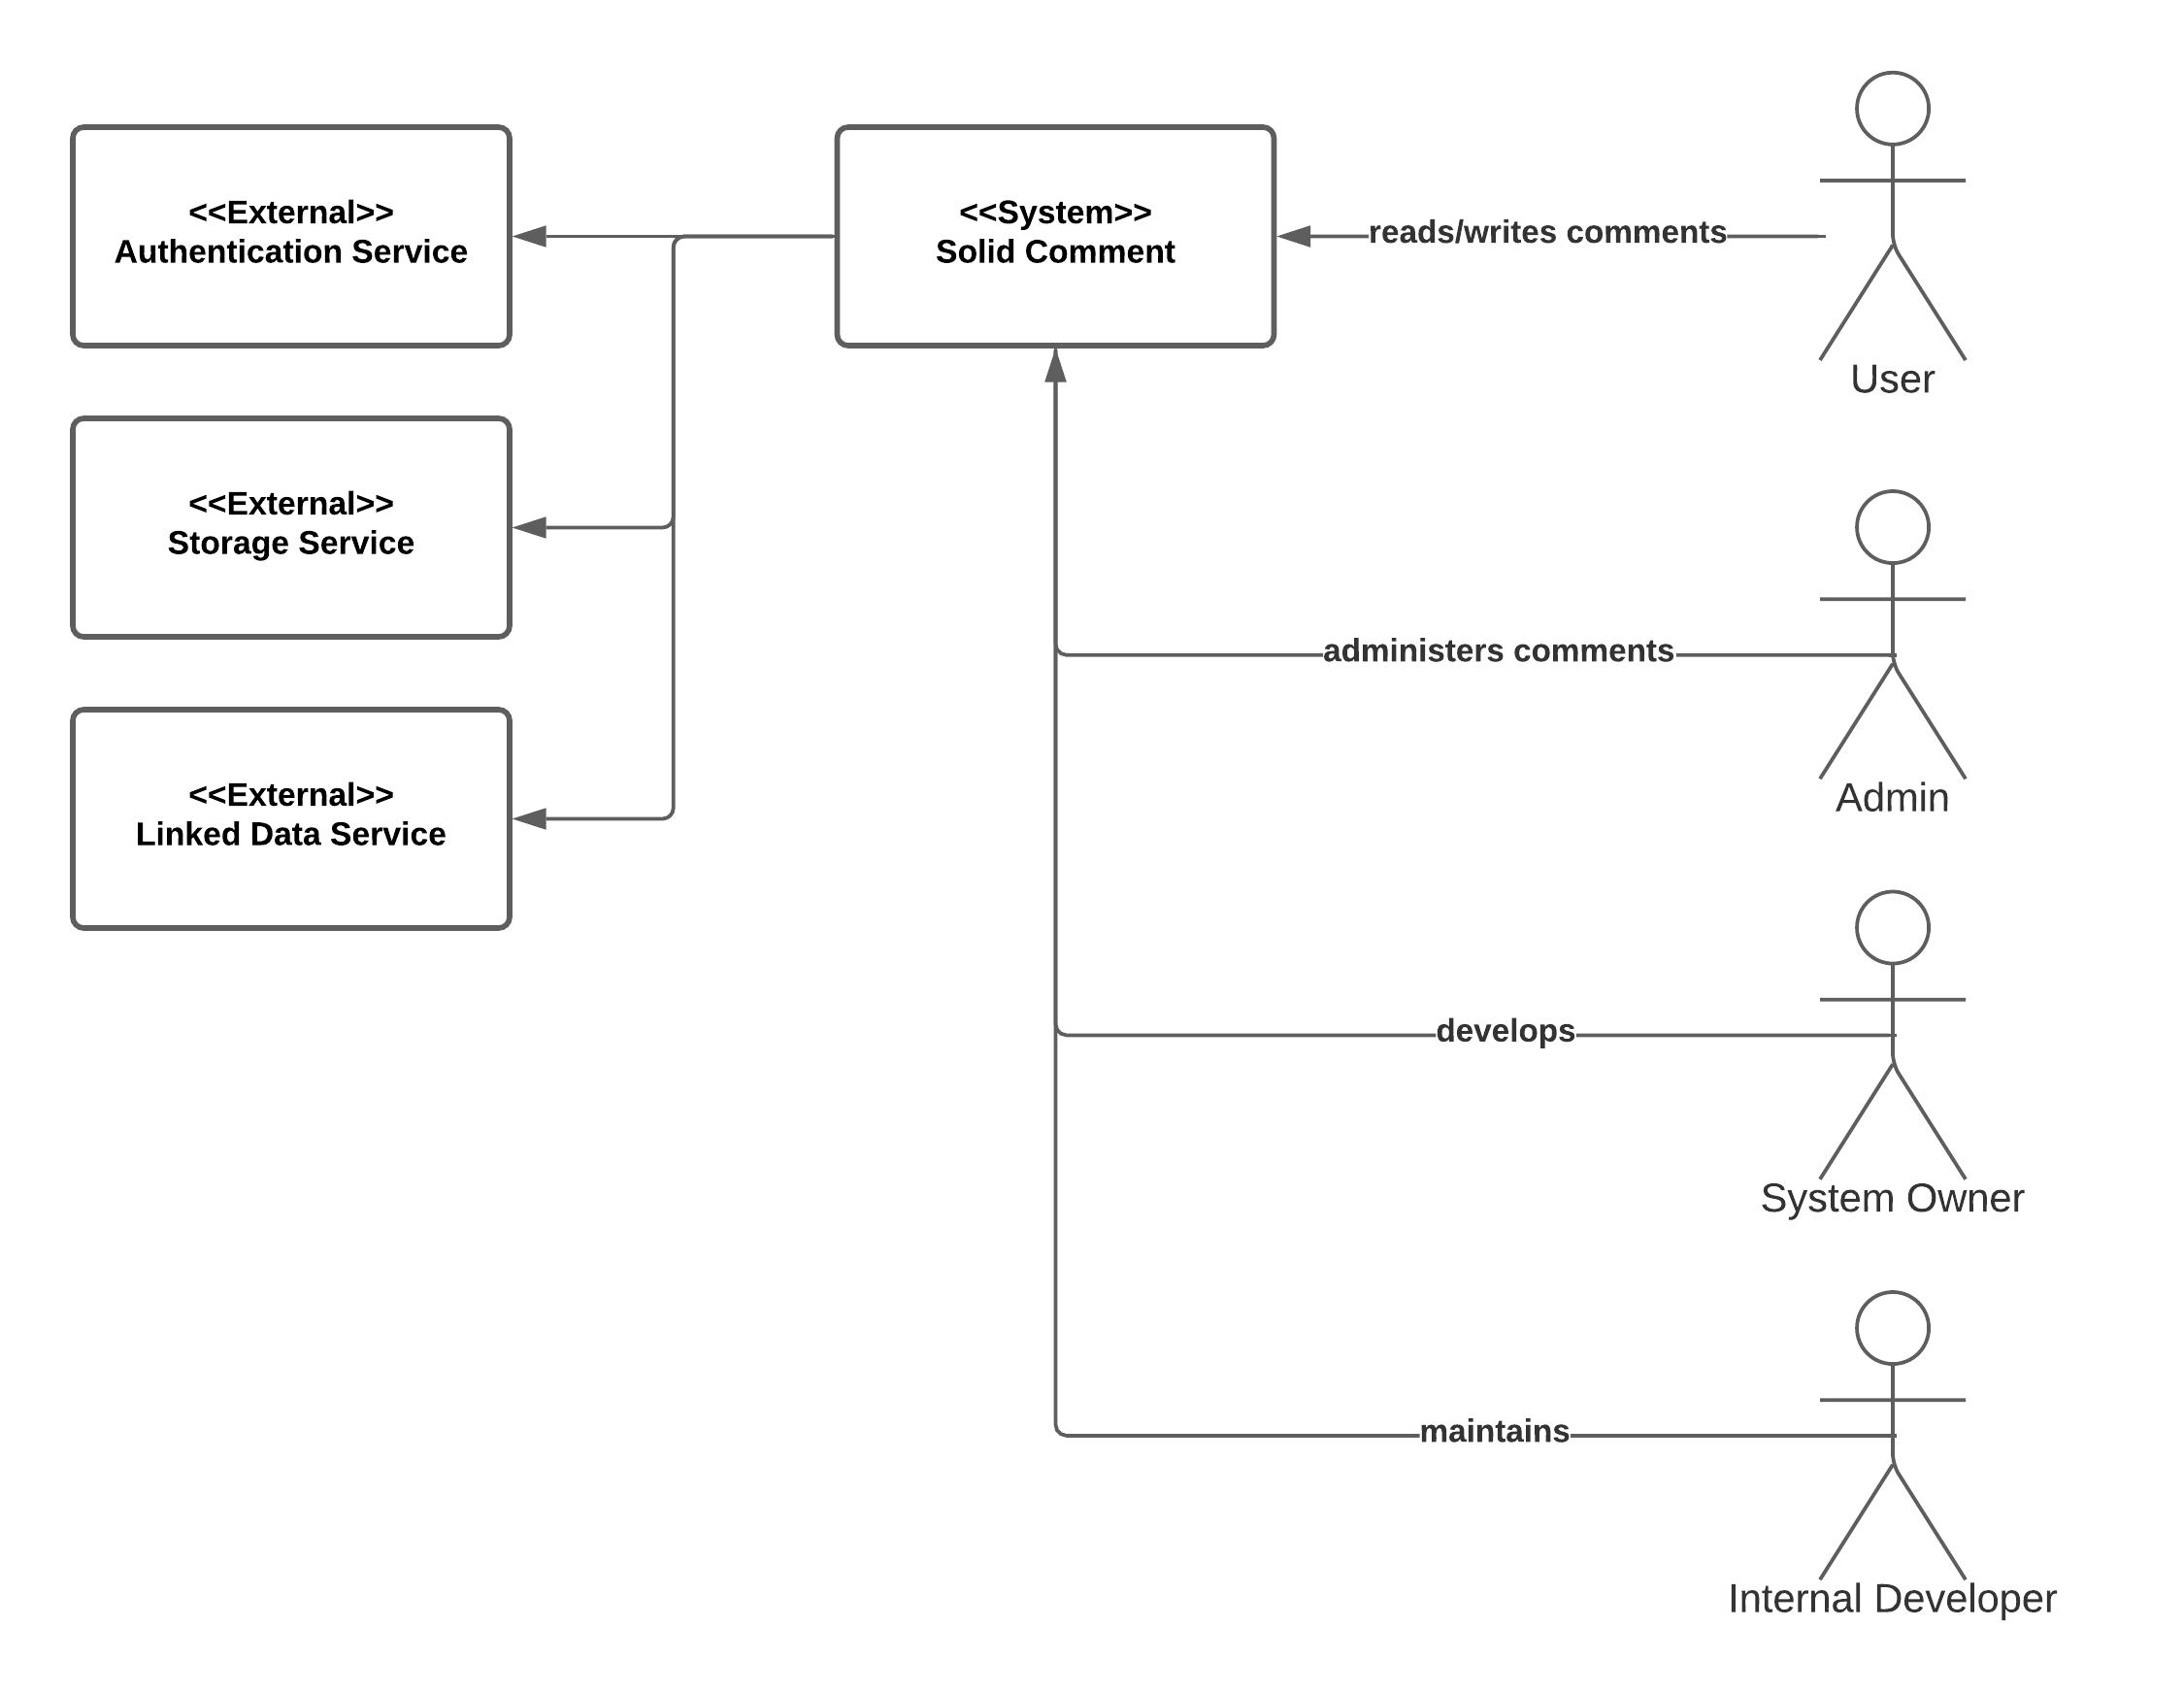
\includegraphics[width=0.8\textwidth]{prototype/graphs/poc-comment-context_diagram.png}
    \caption{Context diagram showing users and external services of the system.}
    \label{fig:poc-comment-context_diagram}
\end{figure}
\vspace{0.5cm}
\paragraph{Sequence Diagram}\mbox{}\\

A sequence diagram brings a suitable overview for any software architecture but especially useful for decentralized systems or those containing several separate services. It gives a clear understanding of each service’s tasks and their relationship when passing messages around in the overall design.

\begin{figure}[H]
    \centering
    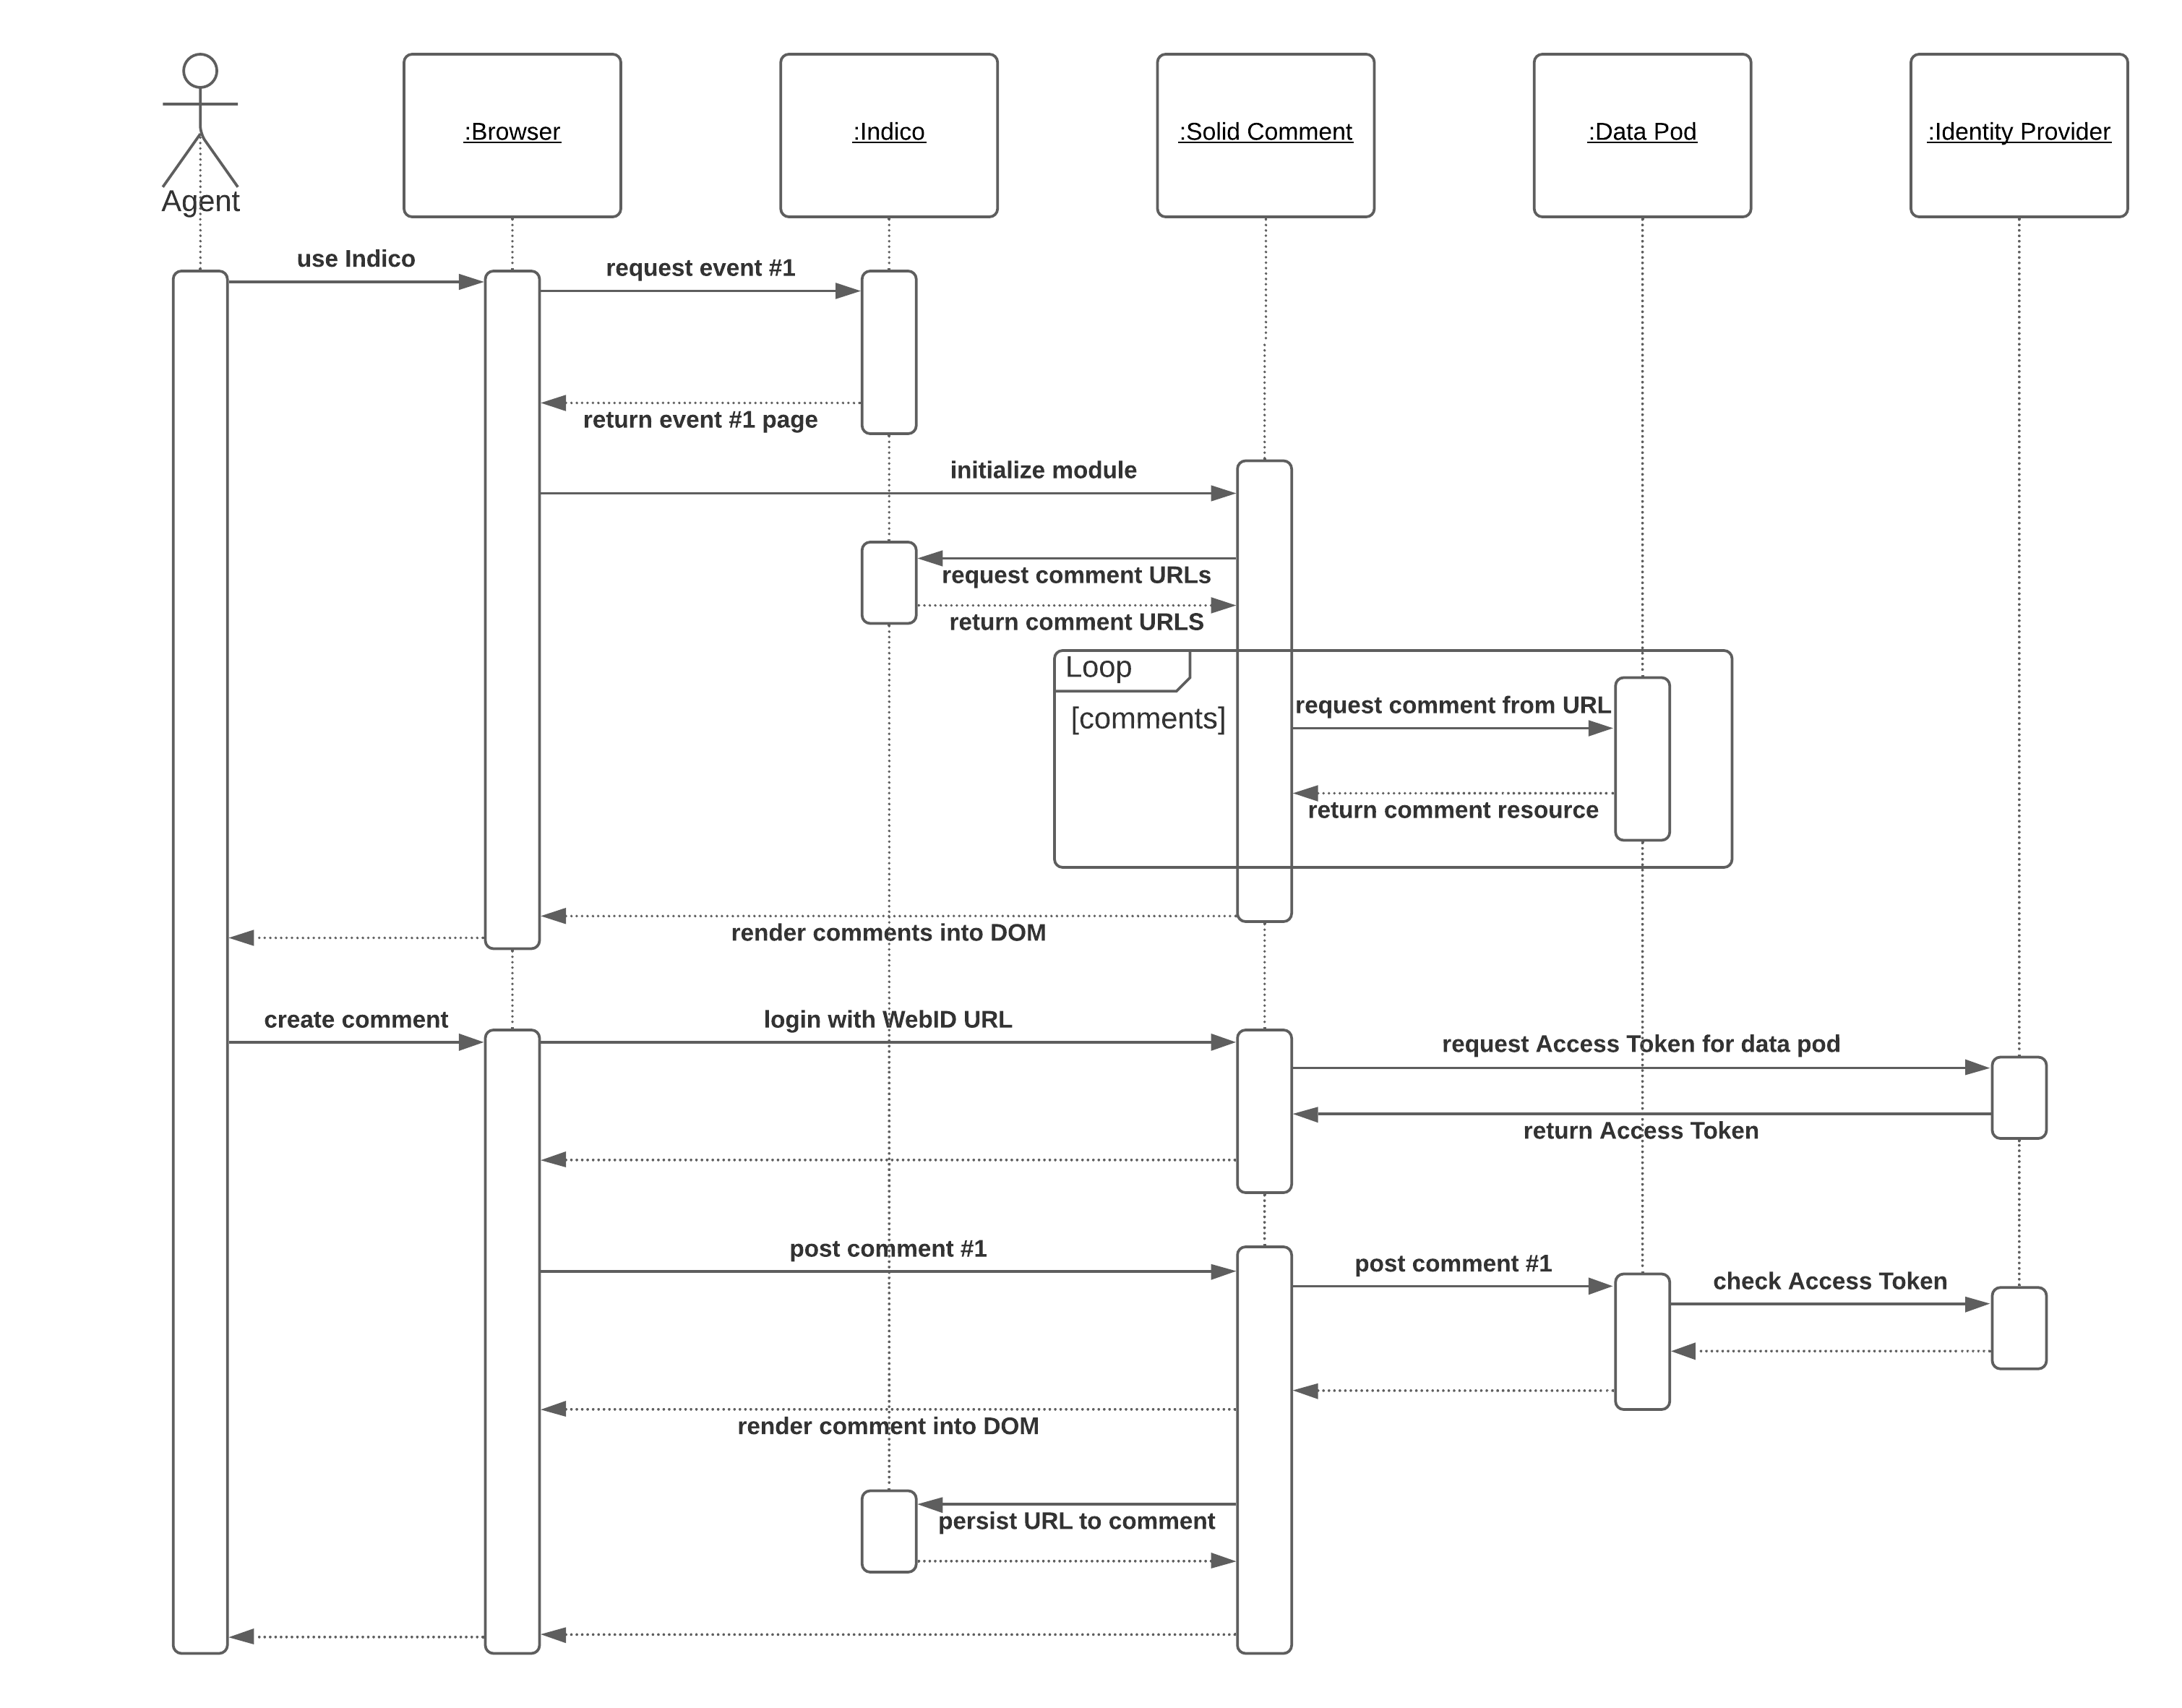
\includegraphics[width=\textwidth]{prototype/graphs/poc-comment-sequence_diagram.png}
    \caption{Sequence diagram showing the sequential process through posting a comment.}
    \label{fig:poc-comment-sequence_diagram}
\end{figure}
\vspace{0.5cm}
\paragraph{Stakeholders}\label{poc1-stakeholders}\mbox{}\\

This section covers the various stakeholders concerning the system. The stakeholders include active users and various external and internal stakeholders impacted by the system or who have a significant say in the development process.

The \textbf{product owner} is responsible for the product, in this case, Indico. Usually, they plan repeated fixed time-boxes in which new features are developed, or the existing software is maintained. They are constantly evaluating the state of the software and try to satisfy other stakeholders such as investors or the system users themselves. The main concerns of the product owner are to stay innovative while no compromising the quality of the existing software.

The \textbf{internal developer} is responsible for executing the decision made by, or together with, the product owner. The developer is also maintaining the software and is the one working with it daily and can make assumptions about the evolution of the software. Their concerns lie in the maintainability of the software through its evolutionary cycle and onboarding new developers.
\vspace{0.5cm}
\paragraph{Drivers}\mbox{}\\

The architectural drivers or \glspl{qa} can be specified using “-illities”. These \glspl{qa} were defined with the stakeholders together in several meetings in which the existing \glspl{qa} of the system, where the \textit{comment} module would be embedded into, were drawn up. \textit{Security} and \textit{Performance} are of utmost priority to the chief developer and product owner. For the collaboration manager, having used Solid for a while, it was clear that the module is usable, requires as little effort as possible, and causes the lowest friction.

\begin{enumerate}
    \item Security
    \item Performance
    \item Usability
\end{enumerate}

\subsubsection{User Interface}\mbox{}\\

For various held meetings and presentations, a visual representation of the to-be-developed module helps guide the audience through the process. For the comment module, a \gls{ui} was designed in graphical software to ease the explanation of the goals for the module. The existing Indico color scheme was adopted to blend into the system.

\begin{figure}
    \centering
    \begin{subfigure}{.5\textwidth}
      \centering
        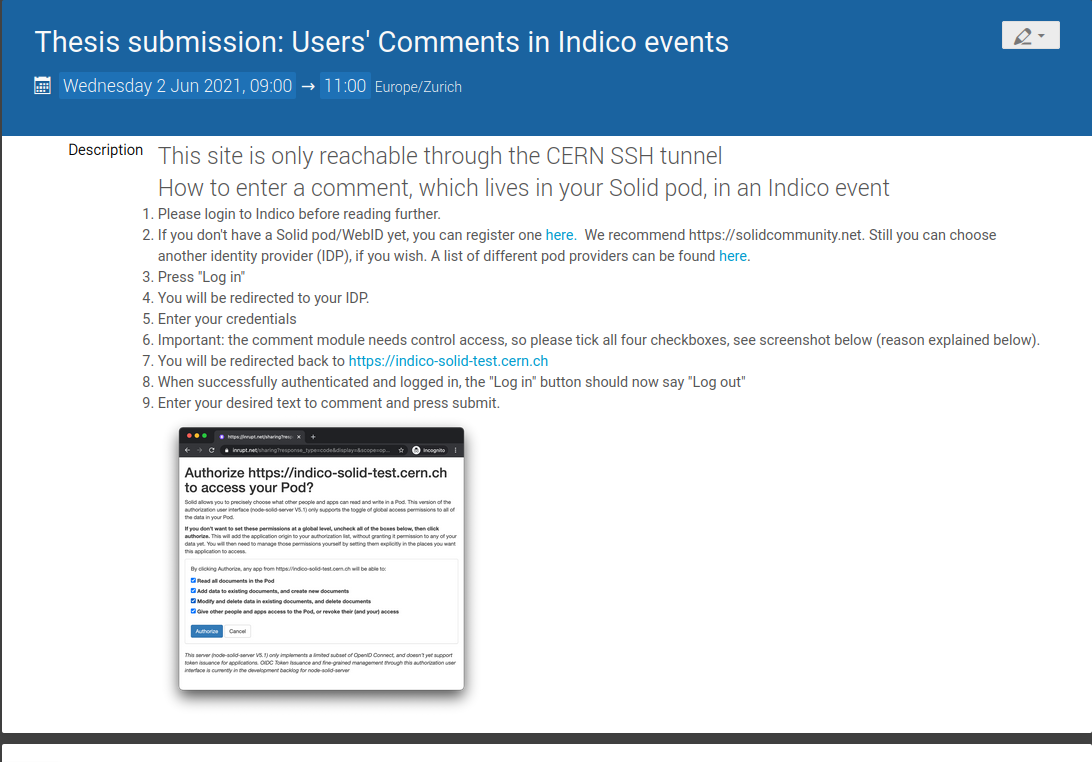
\includegraphics[width=0.9\textwidth]{prototype/poc-solid-comment-description.png}
        \caption{\gls{ui} showing the comment module: Description.}
        \label{fig:poc-solid-comment-description}
    \end{subfigure}%
    \begin{subfigure}{.5\textwidth}
      \centering
    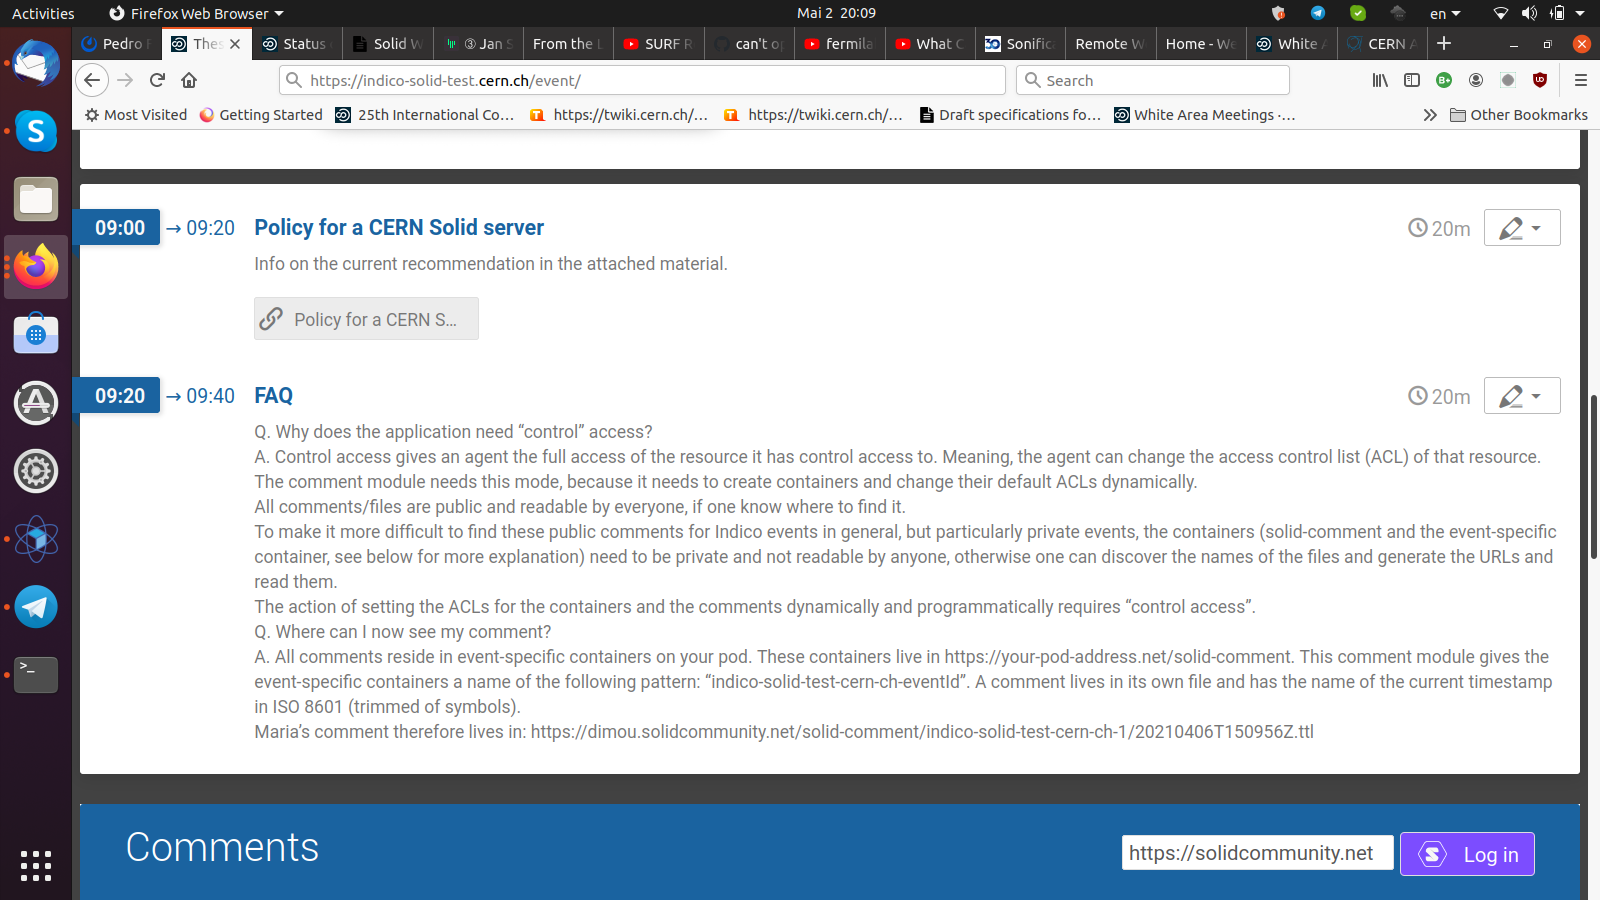
\includegraphics[width=0.9\textwidth]{prototype/poc-solid-comment-agenda.png}
    \caption{\gls{ui} showing the comment module: FAQ.}
    \label{fig:poc-solid-comment-agenda}
    \end{subfigure}
    \caption{\gls{ui} of Indico}
    \label{fig:test}
\end{figure}

\begin{figure}[ht!]
    \centering
    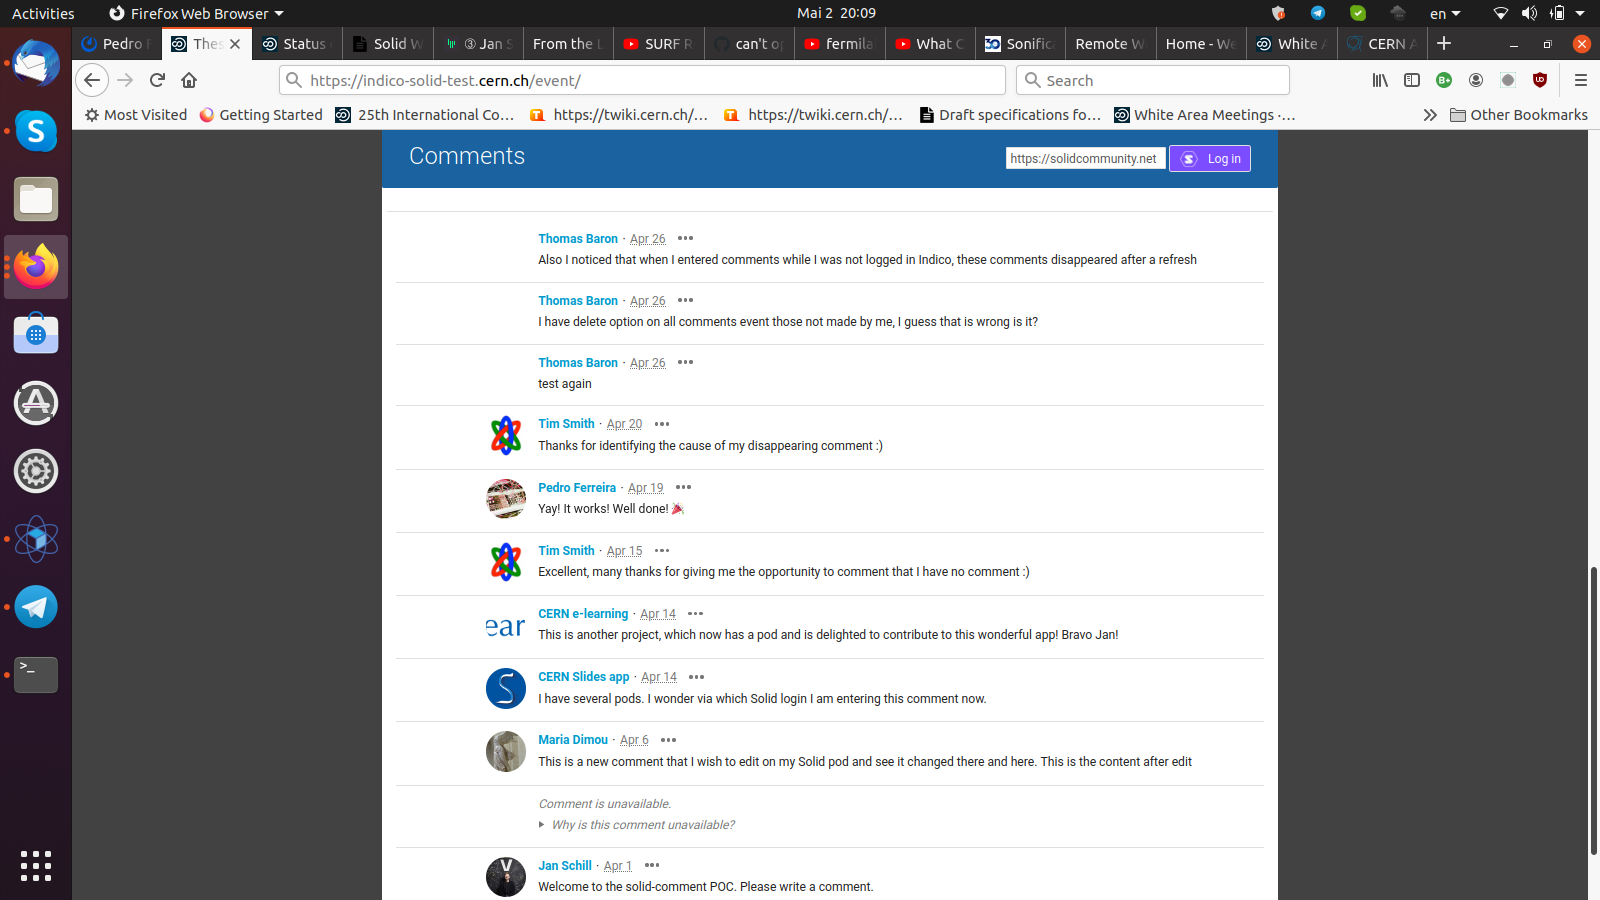
\includegraphics[width=0.5\textwidth]{prototype/poc-solid-comment-comments.png}
    \caption{\gls{ui} showing the comment module: Comments.}
    \label{fig:poc-solid-comment-comments}
\end{figure}

\subsubsection{Design}\label{subsubsection:design}\mbox{}\\

For the implementation of this module, several design decisions had to be made from the fundamental choice of the module running on the client device or be computed on the server and then propagated to the client afterward or even with a microservice proxying all traffic to enable Solid without changing Indico.
Other design challenges were around how to protect the resources holding the comment information. These resources reside on the external data pod and need to be fetched from the application and read by other agents. Can \glspl{acl} be configured to allow the specific use-case and other questions to come up and had to be considered?
\vspace{0.5cm}
\paragraph{Client- Versus Server-Side Versus Microservice}\mbox{}\\

When an agent browses to a running instance of Indico most of the functionality is being prepared on the server hosting Indico. It retrieves the specific request, builds the \gls{html}, and sends it to the user. For Indico most of the functionality is built with Python and the web framework Flask. Sometimes functionality needs to be closer to the user, an example is a dynamic rendering of \gls{dom} elements. Dynamic rendering is useful when new data is shown right away without a blank white screen on a page reload. Indico does send \gls{js}, which is used for client-side features, but it focuses on keeping most of its components on the server.

To make the right decision if the module should be primarily developed for the client- or server-side or even as a microservice, a list of requirements to the module had to be defined. With the specified requirements in place, it had to be figured out how much functionality can be extracted from existing libraries and how much needed to be implemented with the new module. Implementing existing functionality for a new programming language would defeat the \gls{poc}’s purpose of showing how an existing software could work with the Solid principles.

The rudimentary set of features to enable commenting for users in Indico while saving the data in a data pod includes: 
\begin{enumerate}
    \item Authentication with a Solid \gls{idp}
    \item (Authenticated) Requests to a data pod
    \item Parsing of structured data (Linked Data)
\end{enumerate}
\vspace{0.5cm}
\paragraph{Client Approach}\mbox{}\\

The module runs in the browser and is therefore written in \gls{js}. A programming language that compiles to \gls{js}, such as \gls{ts}, is also possible. A browser solution means Indico remains primarily untouched but would have to serve the needed \gls{js} to the client on traffic to an event endpoint where the comment module is integrated.

\begin{table}[h!]
    \centering
    \begin{tabular}{| l | l |} 
     \hline
     Problem & Solution \\
     \hline
      Language & \gls{js} or \gls{ts}  \\
      Framework & Native \gls{js}  \\
      Client & solid-client-js \cite{solid-client-js}  \\
      Authentication & solid-client-authn-browser \cite{solid-client-authn-browser} \\
      RDF & solid-common-vocab-js \cite{solid-common-vocab-js}, rdflib.js \cite{rdflib.js}  \\
     \hline
    \end{tabular}
    \vspace{0.75cm}
    \caption{Existing solutions to problems for a client approach.}
    \label{table:1}
\end{table}

The communication flow with the data pod and the module would happen primarily from the browser.

\begin{figure}[H]
    \centering
    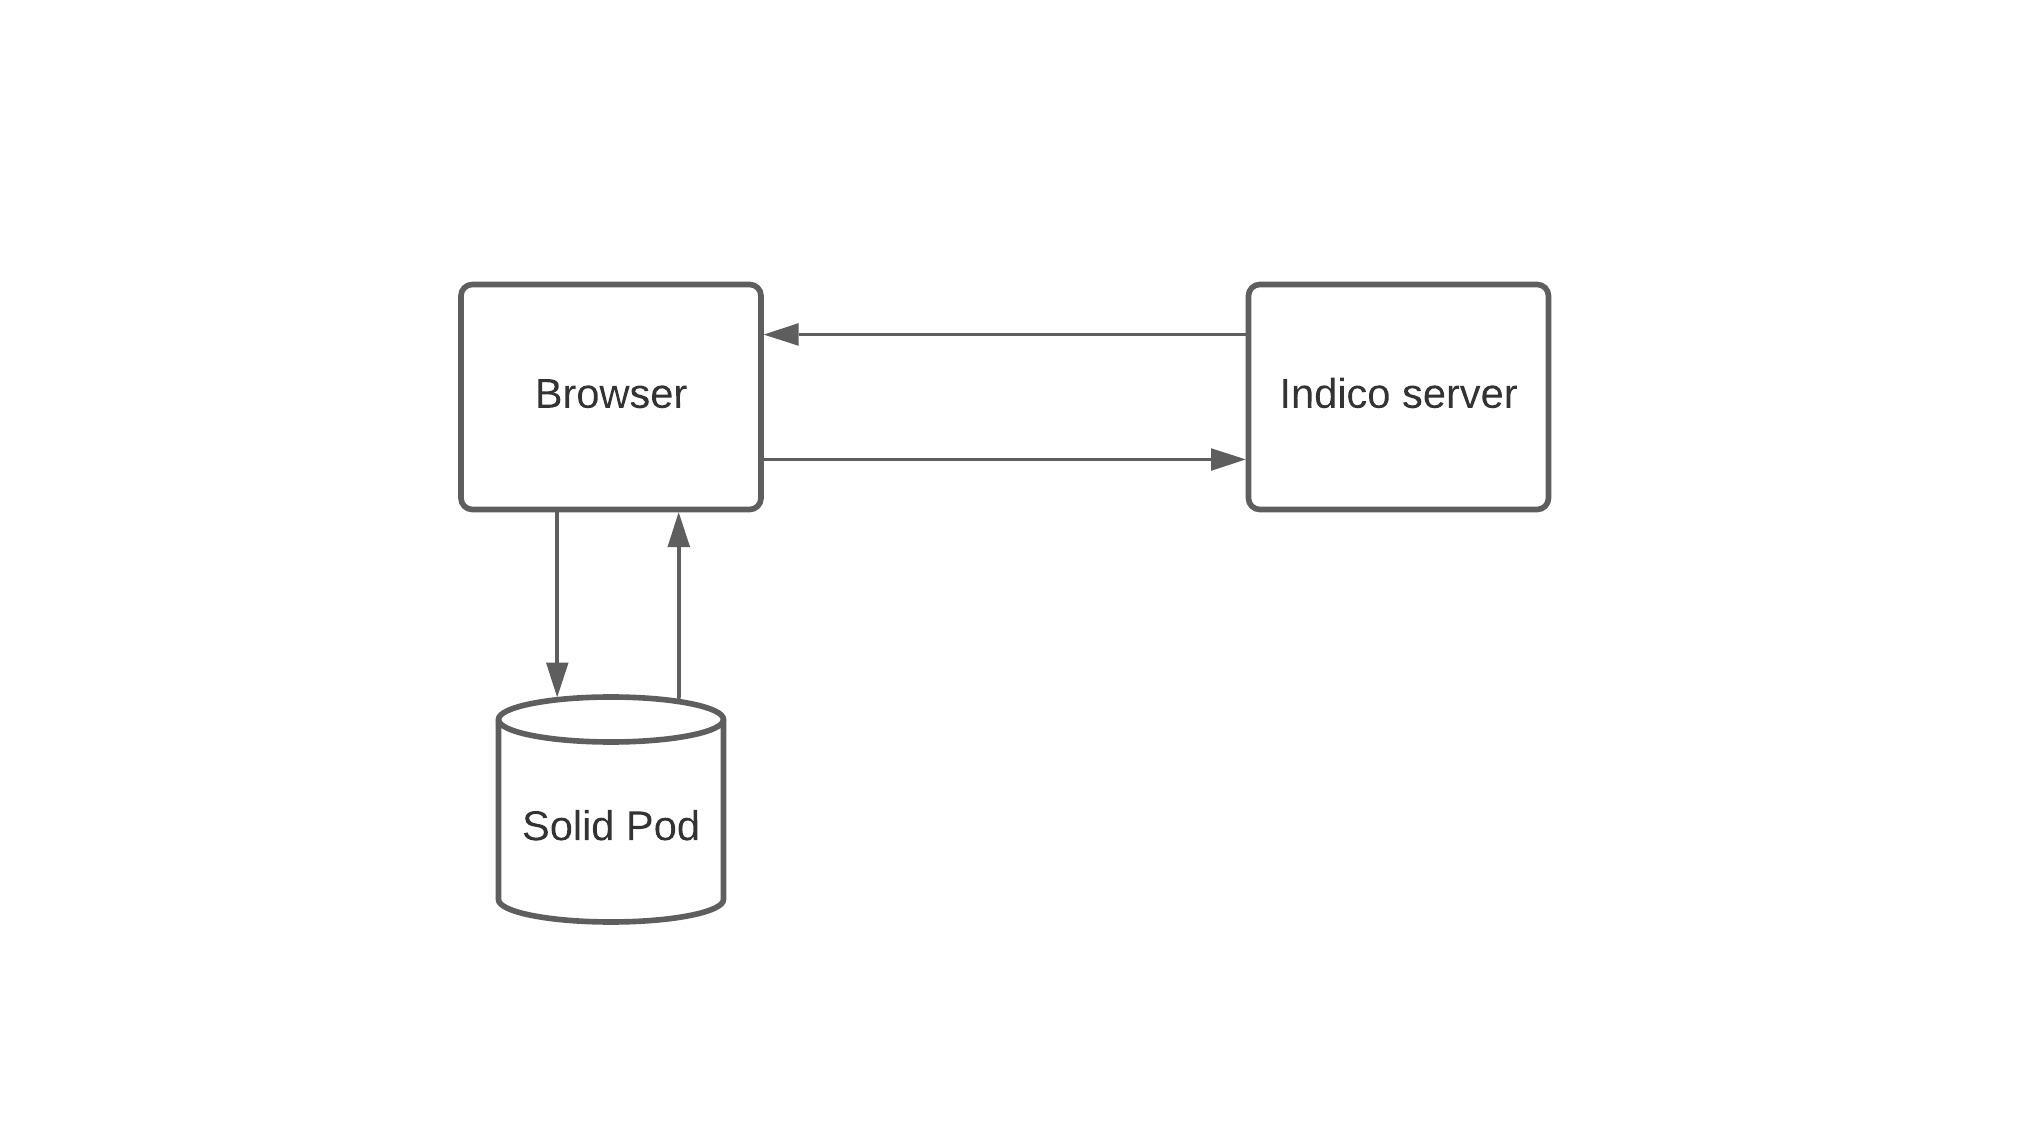
\includegraphics[width=0.8\textwidth]{prototype/graphs/poc-infrastructure-frontend.jpeg}
    \caption{Communication flow for a module developed on the client.}
    \label{fig:poc-infrastructure-frontend}
\end{figure}
\vspace{0.5cm}
\paragraph{Microservice Approach}\mbox{}\\

The microservice approach would allow developing the needed Solid logic on a separate service, which proxies all Solid related traffic and enables the Solid functionality. Most of the libraries from the client implementation can be used as well, as both developments would be written in \gls{js}. Only the authentication flow would work a bit differently.

\begin{table}[h!]
    \centering
    \begin{tabular}{| l | l |} 
    \hline
     Problem & Solution \\
     \hline
      Language & \gls{js} or \gls{ts}  \\
      Framework & Node.js  \\
      Client & solid-client-js \cite{solid-client-js}  \\
      Authentication & solid-client-authn-node \cite{solid-client-authn-node} \\
      RDF & solid-common-vocab-js \cite{solid-common-vocab-js}, rdflib.js \cite{rdflib.js}  \\
    \hline
    \end{tabular}
    \vspace{0.75cm}
    \caption{Existing solutions to problems for a microservice approach.}
    \label{table:2}
\end{table}

The microservice module would handle all requests aimed at the data pod and make it compliant with the Solid server. It would provide the client with the proper \gls{solidoidc} flow to attach the access token to all authenticated requests.

\begin{figure}[H]
    \centering
    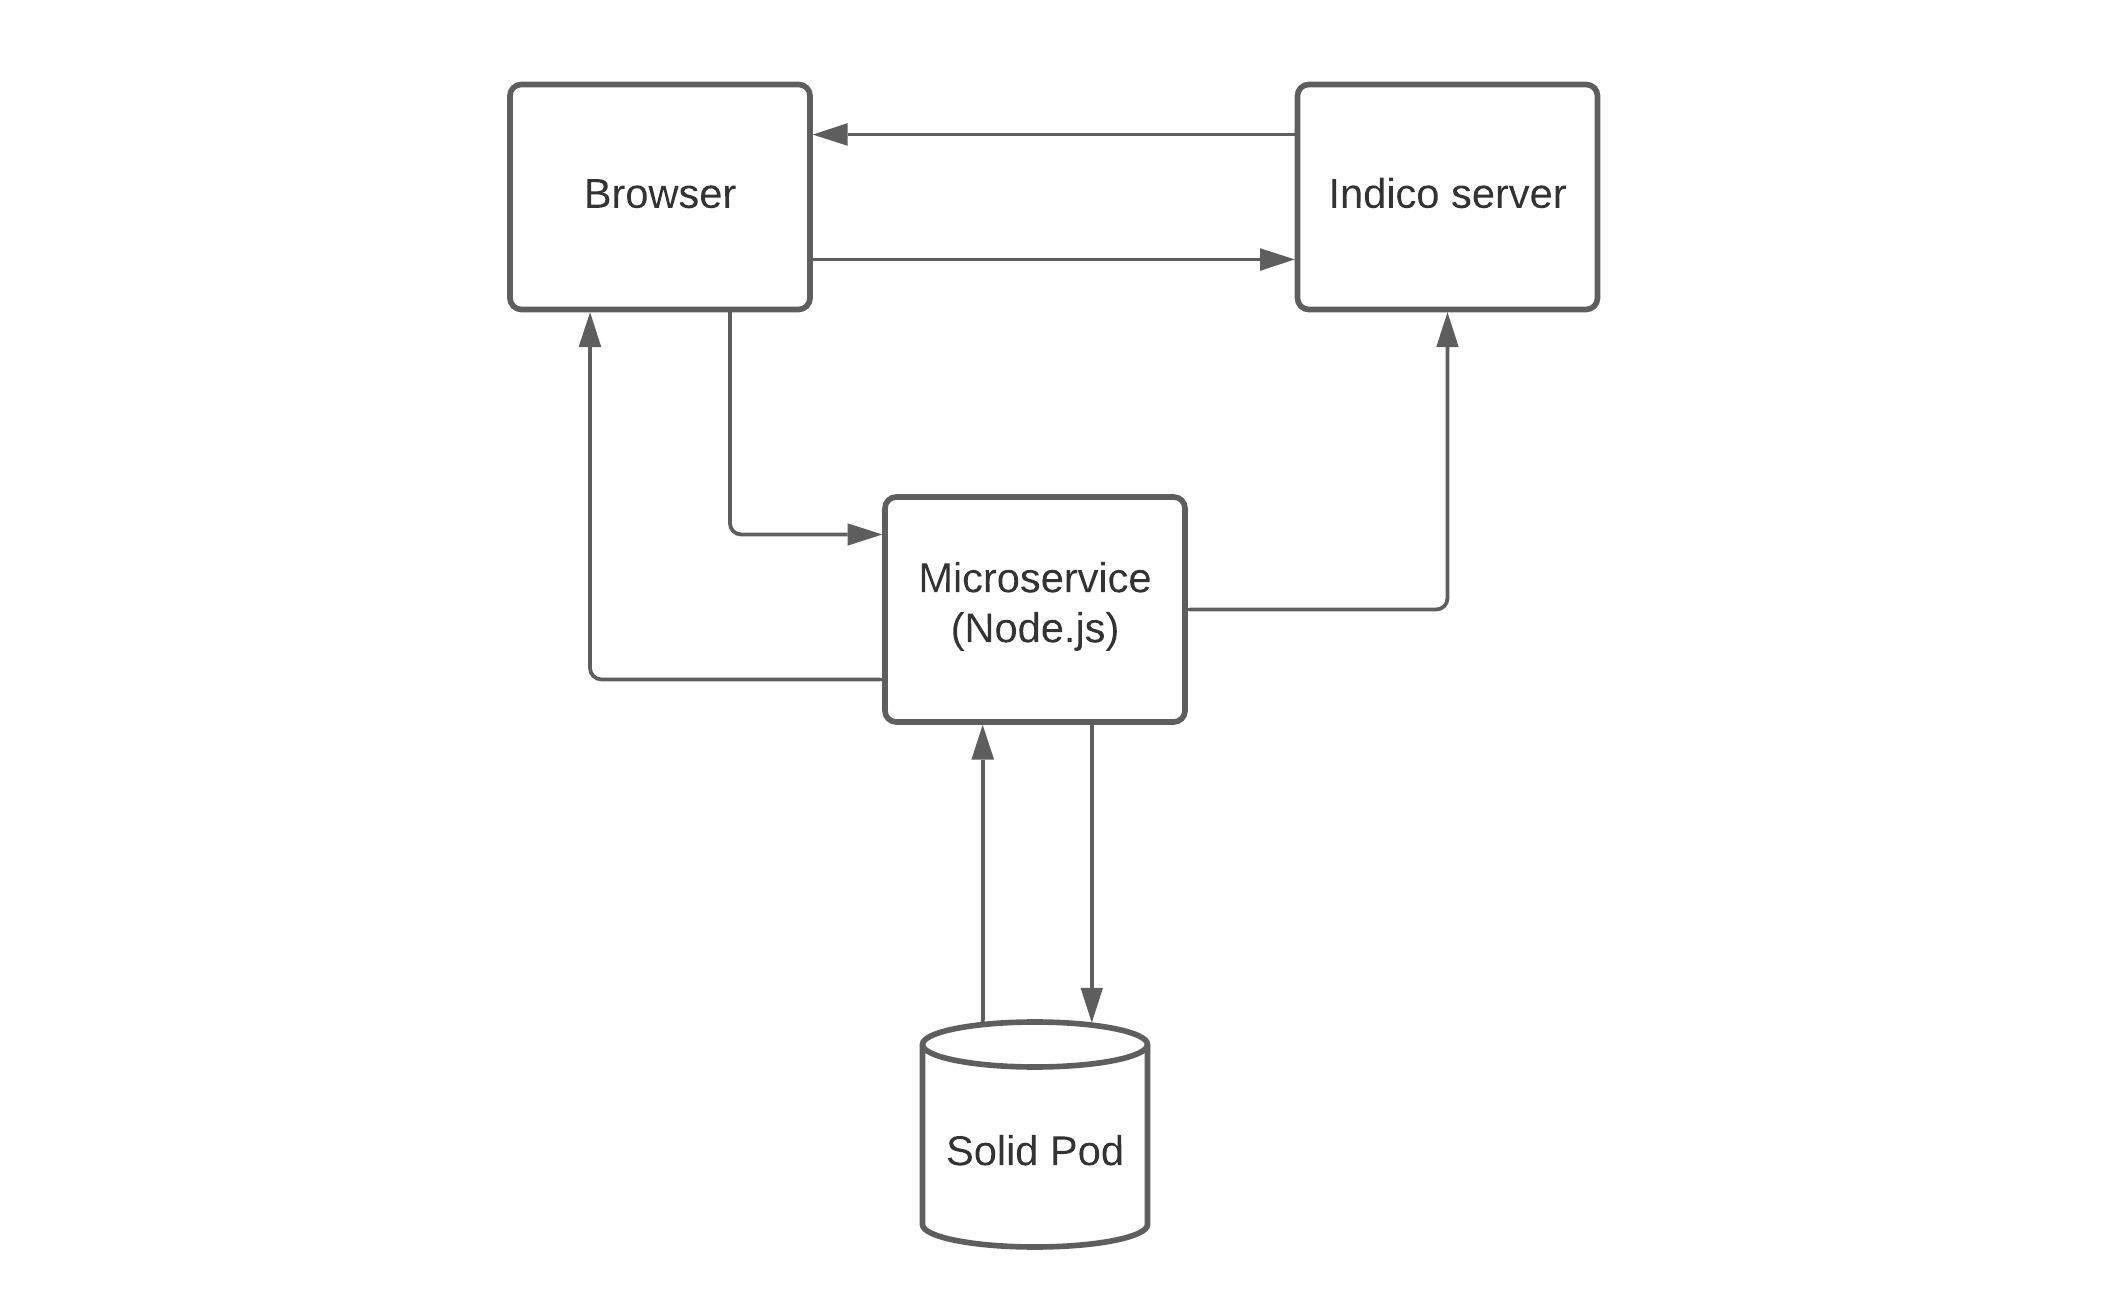
\includegraphics[width=0.8\textwidth]{prototype/graphs/poc-infrastructure-microservice.jpeg}
    \caption{Communication flow for a module developed as a microservice.}
    \label{fig:poc-infrastructure-microservice}
\end{figure}
\vspace{0.5cm}
\paragraph{Server Approach}\mbox{}\\

The goal of the server approach would be just like with the microservice system to decouple the logic needed to work with Solid from the client and have it run on a server instance. The attractiveness for the server approach would be it could be fully integrated within Indico and be part of its Python codebase. Significant drawbacks are no Solid libraries written in Python exist to allow a seamless integration into the ecosystem.

\begin{table}[!ht]
    \centering
    \begin{tabular}{| l | l |} 
    \hline
     Problem & Solution \\
     \hline
      Language & Python  \\
      Framework & Flask  \\
      Client & -  \\
      Authentication & pyoidc \cite{pyoidc} missing DPoP\\
      RDF & solid-common-vocab-js \cite{solid-common-vocab-js}, rdflib.js \cite{rdflib.js}  \\
    \hline
    \end{tabular}
    \vspace{0.75cm}
    \caption{Existing solutions to problems for a server approach.}
    \label{table:3}
\end{table}

The authentication library pyoidc allows authenticating with \gls{oidc} systems but is missing a mandatory feature called \gls{dpop}, which is needed to request protected resources on a data pod. \gls{dpop} is a technique to disallow replay attacks by attaching a \gls{dpop} token to the request indicating what data pod the token can use. In a replay attack, an adversary intercepts the authentication token of an agent and uses the token to make authenticated requests to protected resources. With the usage of \gls{dpop} tokens, the authentication token is signed with a target address. The target address defines the only valid address for which the token can be used. Meaning, when a request is made to a malicious pod, the interceptable token in the \gls{http} header, can only be used to make requests to this data pod and not to any other pods. The \gls{dpop} token therefore needs to be newly generated on everything request \cite{dpop-spec}.

\begin{figure}
    \centering
    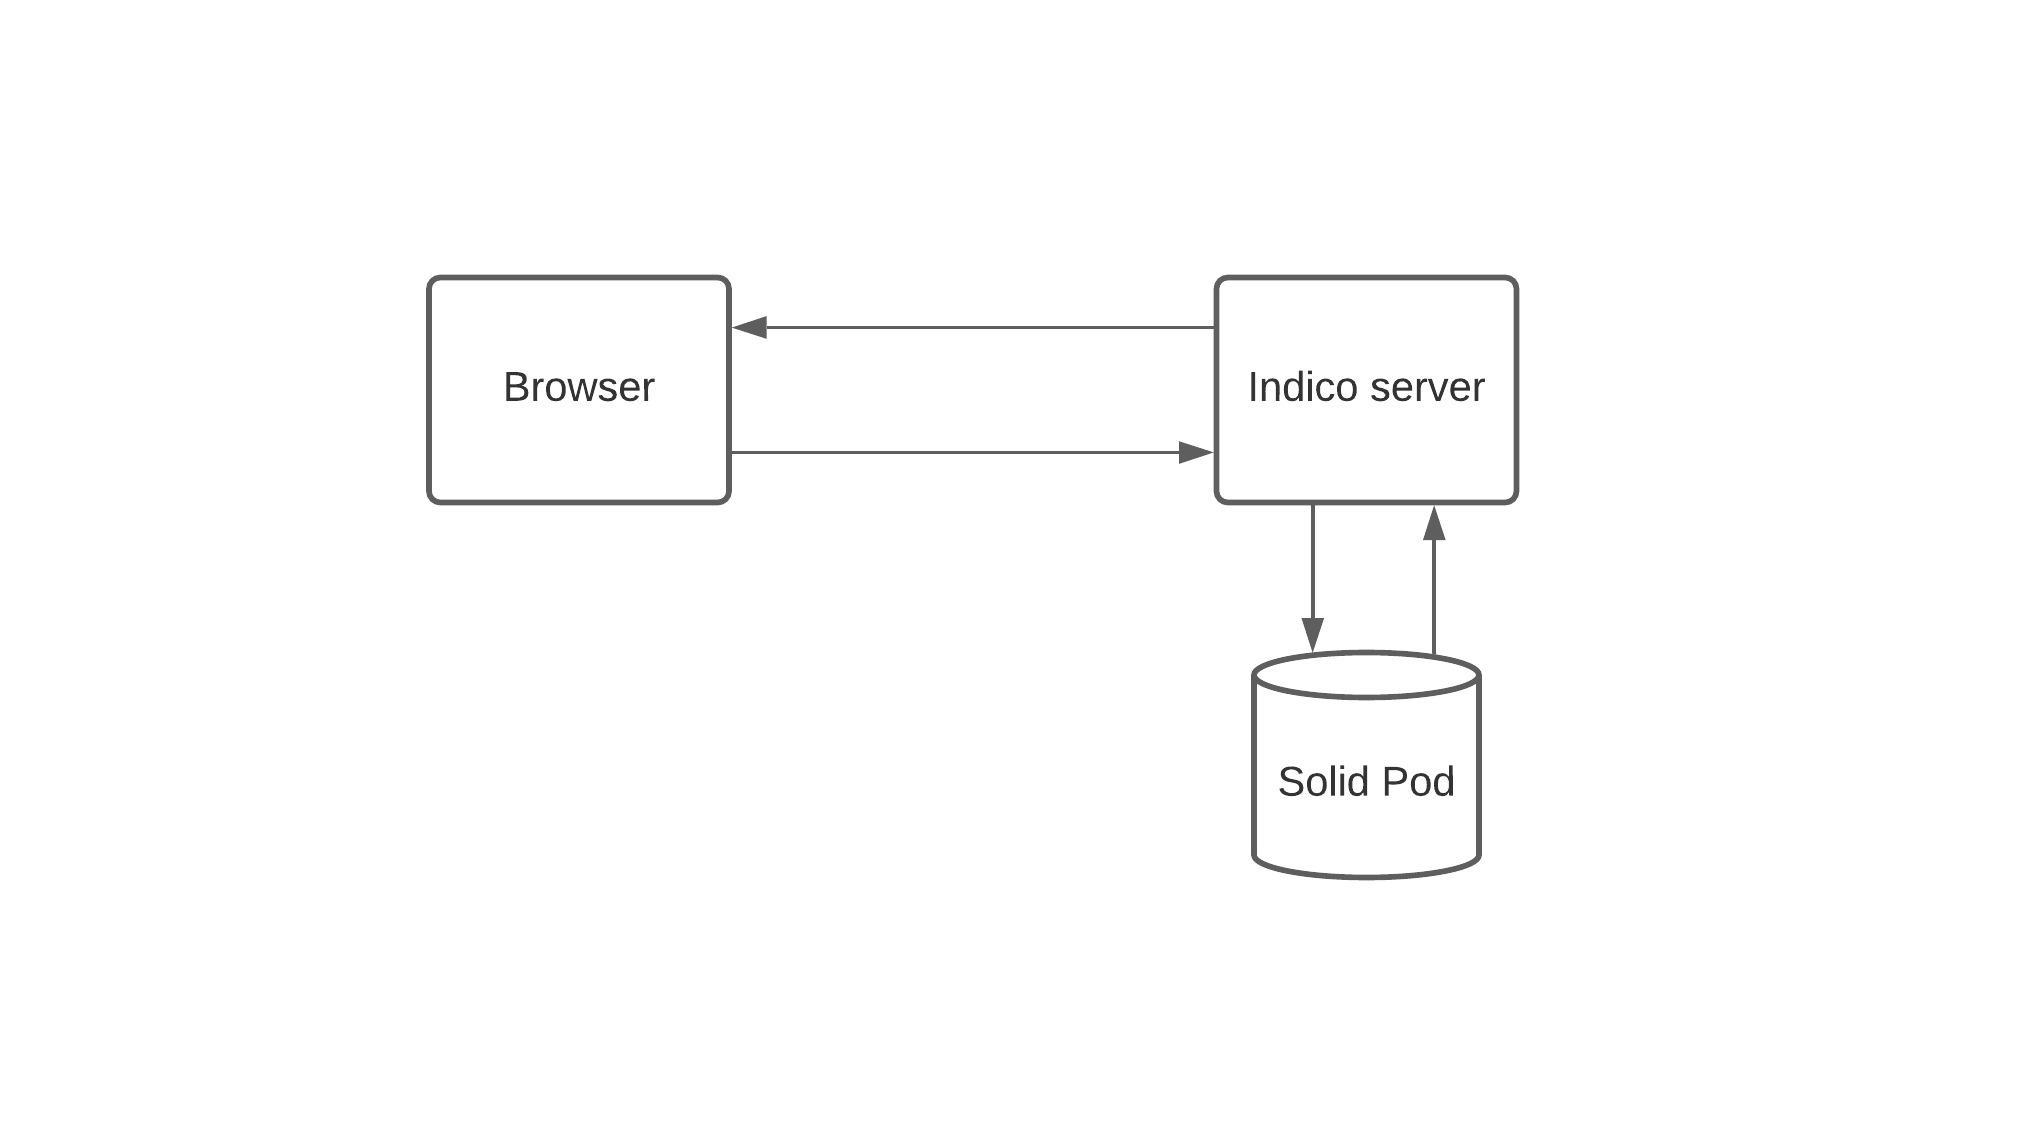
\includegraphics[width=0.8\textwidth]{prototype/graphs/poc-infrastructure-backend.jpeg}
    \caption{Communication flow for a module developed on the server.}
    \label{fig:poc-infrastructure-backend}
\end{figure}
\vspace{0.5cm}
\paragraph{Comparison of the Different Approaches}\mbox{}\\

Benefits from developing the module for the client:

\begin{itemize}
    \item Necessary libraries exist (Major release for all basic Solid flows exist)
    \item Community support
    \item Programming effort for an \gls{mvp} lowest
    \item Documentation on developing Solid apps in \gls{js} exist
\end{itemize}

\begin{table}[h!]
    \centering
    \begin{tabular}{| l | p{11cm} |} 
    \hline
     Library & Description \\
     \hline
      solid-client & A client library for accessing data stored in Solid Pods.  \\
      \hline
      solid-client-authn & A set of libraries for authenticating to Solid identity servers:solid-client-authn-browser for use in a browser.solid-client-authn-node for use in Node.js.  \\
      \hline
      vocab-common-rdf & A library providing convenience objects for many RDF-related identifiers, such as the Person and familyName identifiers from the Schema.org vocabulary from Google, Microsoft and Yahoo!  \\
      \hline
      vocab-solid-common & A library providing convenience objects for many Solid-related identifiers.  \\
      \hline
      vocab-inrupt-common & A library providing convenience objects for Inrupt-related identifiers.  \\
      \hline
    \end{tabular}
    \vspace{0.75cm}
    \caption{Existing solutions to problems for a server approach.}
    \label{table:4}
\end{table}
\vspace{0.5cm}
\paragraph{Single Versus Multiple Resource(s) for Comments}\mbox{}\\

Storing the comments in \gls{rdf} can be done in two ways: holding it in one file as a graph with a list of comments or creating a file for every comment.

\begin{figure}
    \centering
    \begin{subfigure}{.5\textwidth}
      \centering
      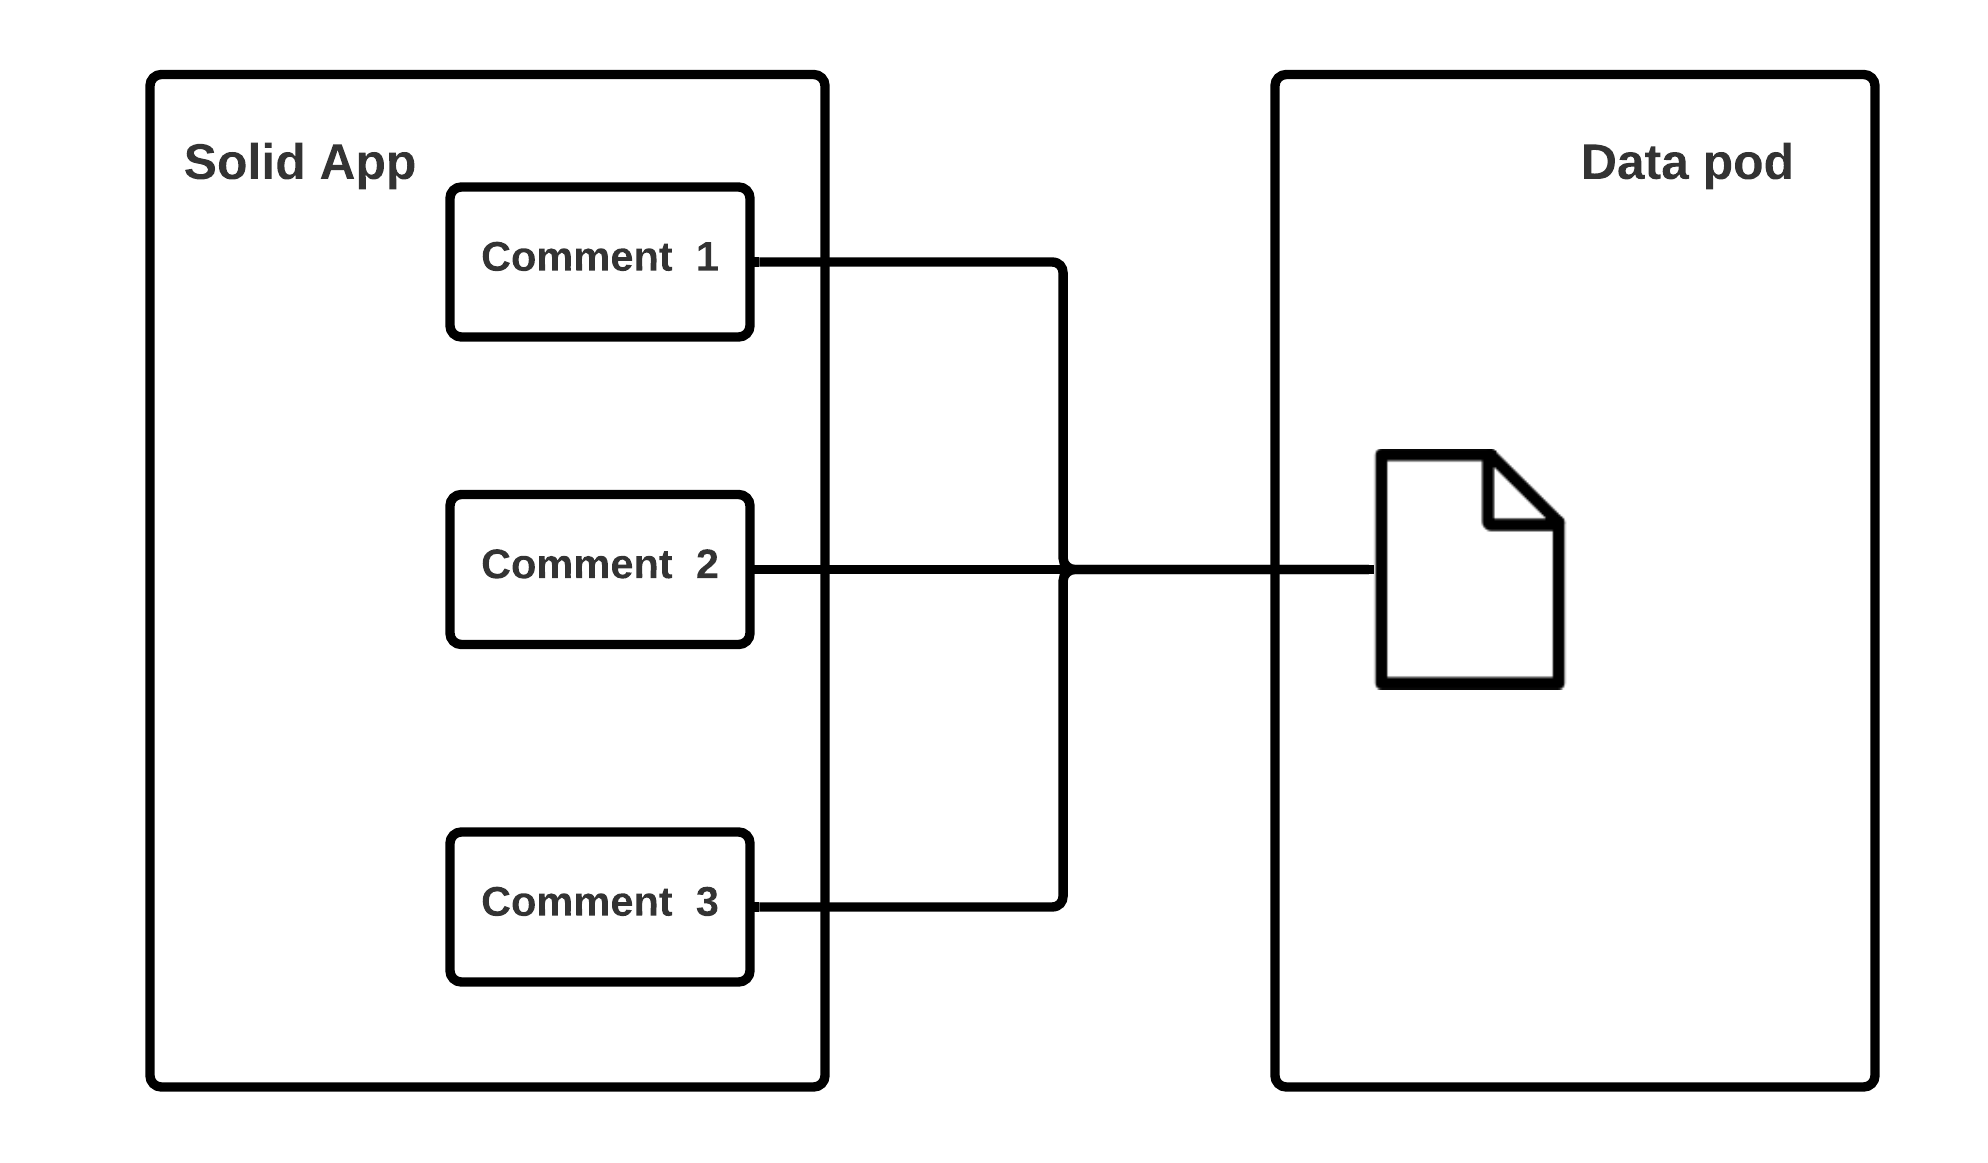
\includegraphics[width=0.7\textwidth]{prototype/graphs/poc-comment-single-resource-comments.png}
      \caption{Comments being written in a single file resource on the data pod.}
      \label{fig:ppc-comment-single-resource-comments}
    \end{subfigure}%
    \begin{subfigure}{.5\textwidth}
      \centering
      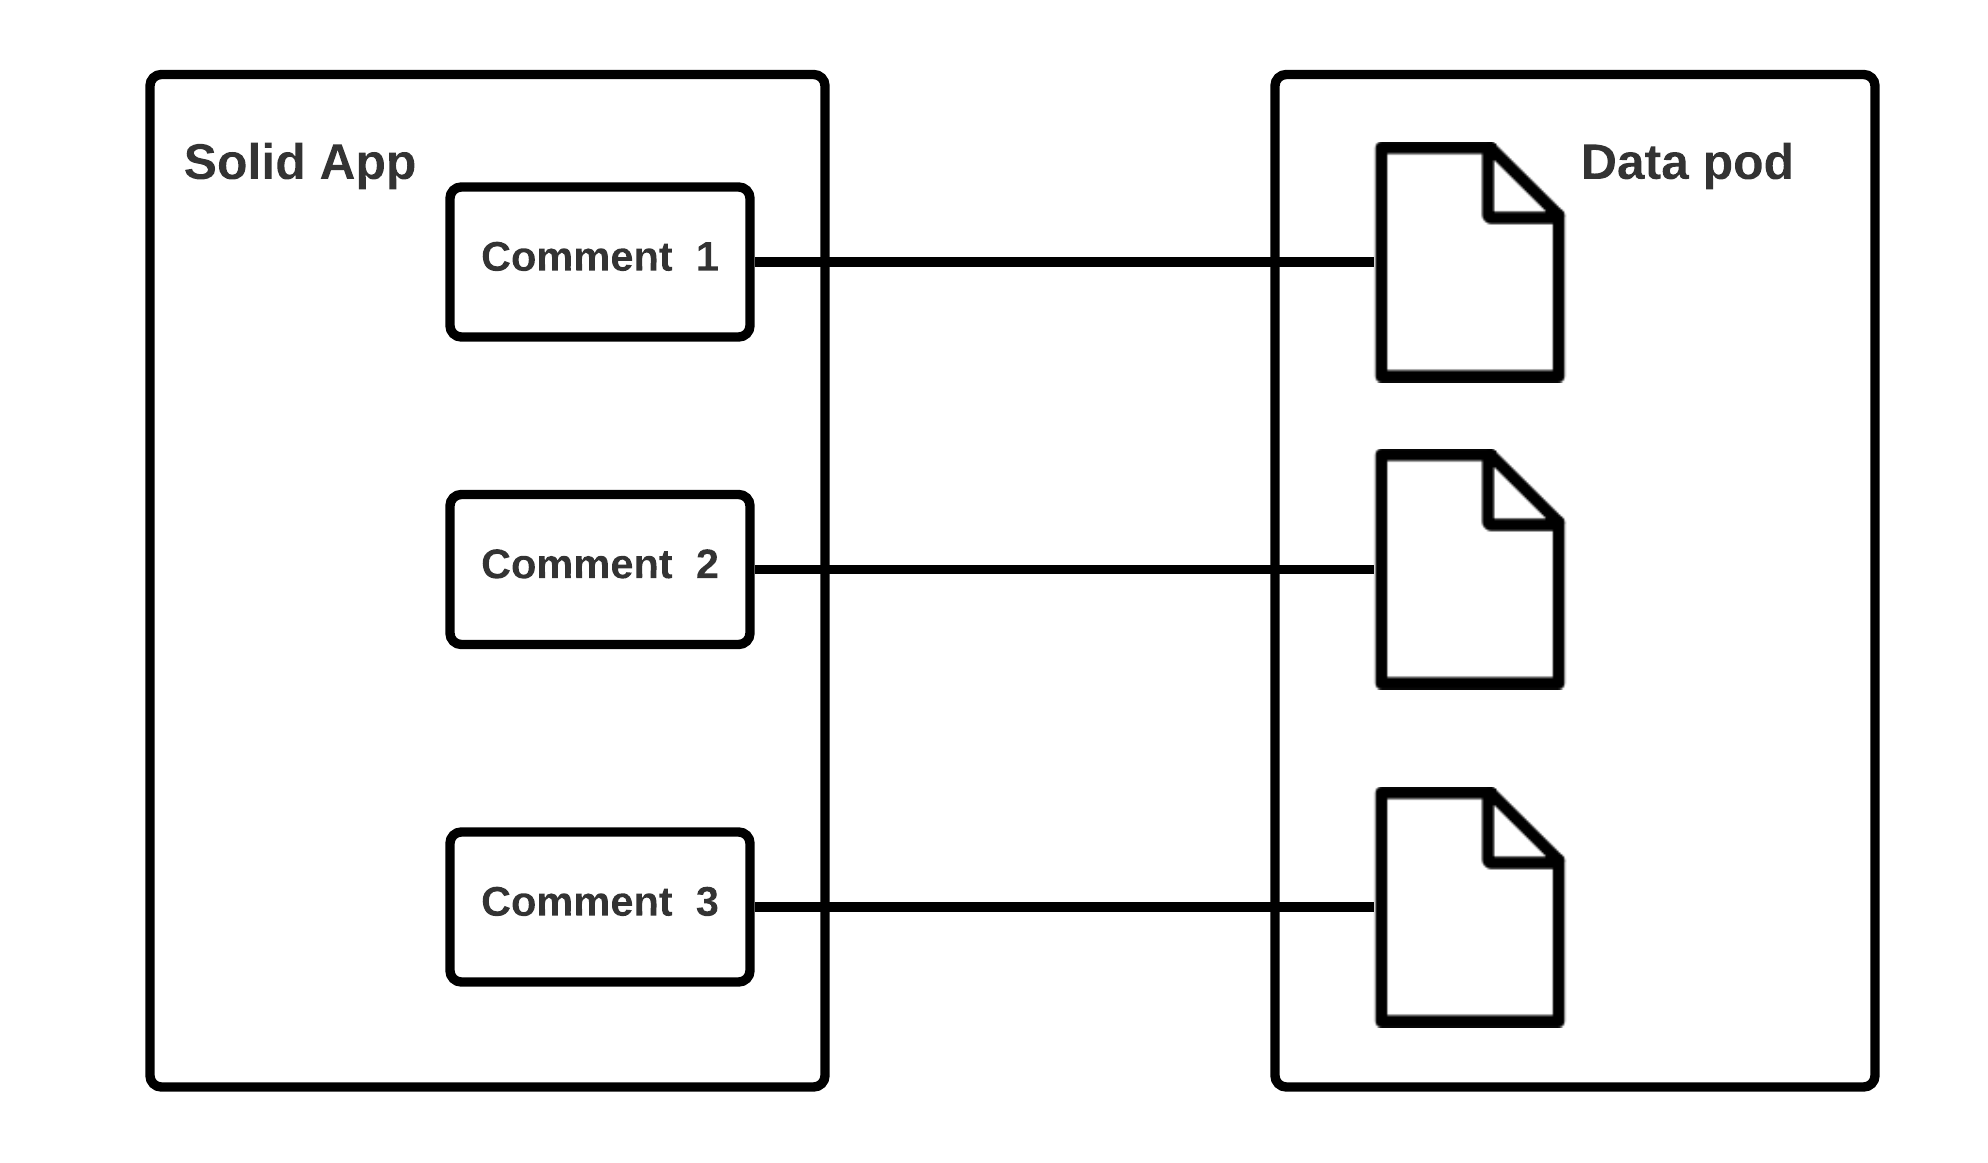
\includegraphics[width=0.7\textwidth]{prototype/graphs/poc-comment-multiple-resources-comments.png}
      \caption{Comments being written in multiple file resources on the data pod.}
      \label{fig:poc-comment-multiple-resources-comments}
    \end{subfigure}
    \caption{Two different ways of saving the comment on the data pod.}
    \label{fig:save-resource}
\end{figure}

When fetching the container with all the comment resources, the request returns a Turtle file describing the container but not the actual content of the contained resources. The misconception of receiving the content was thought to be a problem, as it was assumed an initial request to the container reading its child resources had to be made, and then for each resource, a request needed to be built to retrieve the resource. This overhead was later disproved as the application, where this module is embedded, maintains the list of resources to be fetched. Therefore, no manual building of requests to those resources had to be done. The following paragraph also lays out how this design would not work with the protection of the resources.

\vspace{0.5cm}
\paragraph{Protection on Resource}\label{protection-on-resource}\mbox{}\\

Every container and resource in Solid is protected with \gls{wac}, determining if specific agents, groups, or the world can have read, write, append, or control access. These control access modes are defined in \gls{acl} files. The Solid \gls{acl} inheritance algorithm looks for an \gls{acl} file attached to a specific resource, if it cannot find one, it goes recursively up the file hierarchy and looks for \glspl{acl} on the containers.
Indico allows two general types of protection, \textit{private} and \textit{public}, on its events. Public means open to everyone; no Indico account or authorization is needed to see the event. At the same time, private can be as fine-grained as only to specific agents or groups. A comment module is only valuable if anyone can read and be written by authorized users.

For visitors of a private or public event in Indico to see the comment, the comment’s \gls{acl} needs to allow the public to read the resource.  Public read can be achieved by using the \textit{public} container, which comes with public-read by default on the \gls{nss}, or by creating a new container and setting the \gls{acl} with:

\begin{lstlisting}[language=Other,columns=fullflexible, caption={Setting default read for resources in container}, label={lst:container-acl}]
@prefix acl: <http://www.w3.org/ns/auth/acl#>.
@prefix foaf: <http://xmlns.com/foaf/0.1/>.

# ... Definition for owner

<#example-container-name>
    a acl:Authorization;
    acl:agentClass foaf:Agent;
    acl:accessTo <./>;
    acl:mode acl:Read.
\end{lstlisting}

Every resource in this container is by definition readable by the public -- if not otherwise stated in a more detailed resource \gls{acl}. The above description even allows reading the container’s content, meaning a request to the container would yield a list of resources in the container. A publicly readable list becomes unpleasant if the Indico event is private and the comments for this Indico event should not be read by the world, which is entirely possible when browsing to the location of a specific data pod and then looking into the public container.

An \gls{acl} defining private access to a container can prevent the problem of a random agent seeing a container's content, with the container's resources still public. The private access mode would allow everyone, provided they have the \gls{url}, to read a resource in a private container but not look into the resource’s parent container. To achieve this behavior with \gls{acl}, the container needs to define its owner and no specific rules for the public, as \gls{wac} comes with a default private access control. Each child resource needs to define an \gls{acl} now, allowing public read.
The container’s \gls{acl} would look like the following with just an owner specified:

\begin{lstlisting}[language=Other,columns=fullflexible, caption={Container \gls{acl} with owner defined.}, label={lst:container-acl-owner}]
@prefix acl: <http://www.w3.org/ns/auth/acl#>.

<#owner>
    a acl:Authorization;
    acl:agent <https://janschill.net/profile/card#me>;
    acl:accessTo <./>;
    acl:default <./>;
    acl:mode acl:Read, acl:Write, acl:Control.
\end{lstlisting}

A child resource would allow public read with:

\begin{lstlisting}[language=Other,columns=fullflexible, caption={Giving read mode to child resources}, label={lst:container-acl-read}]
@prefix : <#>.
@prefix acl: <http://www.w3.org/ns/auth/acl#>.
@prefix foaf: <http://xmlns.com/foaf/0.1/>.

# ... Definition for owner

:Read
    a acl:Authorization;
    acl:accessTo <test.txt>;
    acl:agentClass foaf:Agent;
    acl:mode n0:Read.
\end{lstlisting}

Another approach and implemented after iterating through the previous ones is to have the container’s \gls{acl} resource define a default access mode for its child resources. This way, one \gls{acl} only needs to be created on the container, and all resources have proper access modes for public read and are not listed publicly in the container’s description.

\begin{lstlisting}[language=Other,columns=fullflexible, caption={Giving default read mode to all child resources of container.}, label={lst:container-acl-read-default}]
@prefix acl: <http://www.w3.org/ns/auth/acl#>.
@prefix foaf: <http://xmlns.com/foaf/0.1/>.
@prefix target: <./>.

:ReadDefault
    a acl:Authorization;
    acl:default target:;
    acl:agentClass foaf:Agent;
    acl:mode acl:Read.
\end{lstlisting}
\vspace{0.5cm}
\paragraph{Preventing Unwanted Discovery for Resources}\mbox{}\\

With the resources having proper access modes but being publicly readable, a simple naming convention of taking the \gls{iso} 8601 string and using it as a filename for the resources created on the data pod does not suffice -- even though it is a good strategy when looking for a reliable naming convention to prevent duplication. 
Considering performance improvements such as pagination for future iterations of the module, which would require some iterative indication, a combination of randomness, and an order indicator, it was settled for using \gls{uuid} plus the \gls{iso} 8601 string to form a filename.

Other ideas included hashing a random string with the timestamp to generate non-guessable filenames. The filename would need to use the same hash function to decipher the filename to figure out when the comment was generated. \gls{uuid} is a reliable and easy-to-use system to generate \textit{truly} globally unique strings. 
\vspace{0.5cm}
\paragraph{Modification of Resource From Data Pod}\mbox{}\\

When the users control their data, they can revoke access or even change their data to their liking. The ability to modify data from within the data pod means the application cannot be guaranteed the same comment that was initially created and needs to be aware that data can be changed at any time. Even if the system's interface does not allow modification, a modification can still happen at the source of the storage of the comment.

Regular comment modules usually allow updates of a submitted text throughout its existence. Twitter is an example where an update is not allowed after posting \cite{twitter-edit}. 

When the development discovered this aspect, the relevant stakeholders and developer decided to allow this behavior, as it seems natural to edit one's comments.

\vspace{0.5cm}
\paragraph{Mitigation of Spam}\mbox{}\\

Enabling user input in the form of a comment module without application authentication is a spam gateway. Even though authentication with a Solid \gls{idp} is necessary, it does not hinder a malicious actor from creating many Solid accounts and spam into the application. In the first iteration of the module, only Solid authentication was integrated into the module. Therefore, it would allow anyone with a Solid account to post comments and spam the Indico event theoretically. Another authentication layer was added in a second iteration of the module to mitigate spam from outside Indico. For \gls{cern}’s use case, an authenticated Indico session was enough. An Indico session adds an extra step to the comment process, ensuring only registered Indico users can comment.
\vspace{0.5cm}
\paragraph{Giving Application Full Control of Data Pod}\mbox{}\\

An agent or application requires \textit{control} access to the container to create or change \glspl{acl} programmatically in this container. By default, \gls{nss} asks for the permissions when authenticating for the first time in the \gls{solidoidc} flow between the \textit{solid-comment} module and Solid \gls{idp}. The permissions granted to the application are on the root container of the data pod. Giving an application control access allows the application to read, write, change \glspl{acl} on the entire data pod. As a simple application, this is troubling as a commenting module needs to have control access to set the necessary \glspl{acl} for the containers and resources it creates.

The current implementation has not a built-in solution. Still, one way of solving it is using an application launcher, an application itself with complete control access, and then limiting the access controls of the solid-comment module by creating a dedicated container for it and setting the needed \gls{acl} for it this specific container only. 

\subsubsection{Integration with Indico}\mbox{}\\

The need for integration with Indico is twofold: serving the module to the client and being the provider to the list of references to the comments posted on a specific event.
\vspace{0.5cm}
\paragraph{Storing Reference to Comments in Indico}\mbox{}\\

Indico operates using the relational database PostgreSQL \cite{postgresql}. When a comment gets posted and stored on an external data pod, a reference to the location of the comment needs to be kept for Indico to pull the comment and render it in its frontend. Several possibilities are imaginable. 

\begin{enumerate}
    \item Create a new EventComments table
    \item Store in an Indico data pod 
    \item Use the existing EventSettings table
\end{enumerate}

One solution would be to create a new database table that associates with the event using a foreign key and the event id and then stores every comment in its row with all necessary meta information. The database schema would have to be updated to register the new table properly and then executed. A quicker alternative to this is the usage of an existing database table called \texttt{EventSettings}. \texttt{EventSettings} is for additional information for an event and is meant to be a lightweight key-value store for these extra data (often used with Indico plugins).

Another option would be to leave the database alone and embrace the Solid way of storing the comment references by deploying an Indico Solid data pod. The data pod could hold a resource for every event and link to the data pods where the comments reside. This solution is the most aligned with the Solid principles and could have been an interesting challenge to develop, but it was identified too late to push through.
\vspace{0.5cm}
\paragraph{Enforce Authenticated Session For Posting Comments}\mbox{}\\

It was established through the iterations of the design with the stakeholders that an authenticated Indico session is deemed necessary in addition to the already authenticated Solid \gls{idp} session with the data pod. The primary motivation was to keep it as laborious as possible for spam to reach the system.

The awkwardness of validating a current Indico session and then sending requests to a protected endpoint comes with the great decoupling of the comment module and Indico, which is admirable and makes this feature more challenging to implement. Indico uses a framework called Axios \cite{axios} for its \gls{http} client request handling. In Indico Axios, is configured with all necessary \gls{http} headers and, when a session exists, also equipped with the auth-token. The comment module can be extended to allow a custom \gls{http} client to send requests to Indico. When the module is initialized, the Axios client is already readily configured and needs to be passed over to the module. Both systems are still decoupled, and the comment module works with or without a custom \gls{http} client.
\vspace{0.5cm}
\subsubsection{Evaluation}\label{section:poc1-evaluation}\mbox{}\\

This section focuses on evaluating the system. The evaluation shall be done by iterating through the stakeholders' requirements and how the architecture lives up to those expectations. The assessment is done with the help of the \gls{asqa} framework to ensure continuous quality assessment and prioritizing with a lightweight technique \cite{asqa-paper}. \gls{asqa} contains seven process steps, as shown in figure \ref{fig:asqa-process-steps}.

\begin{figure}[!ht]
    \centering
    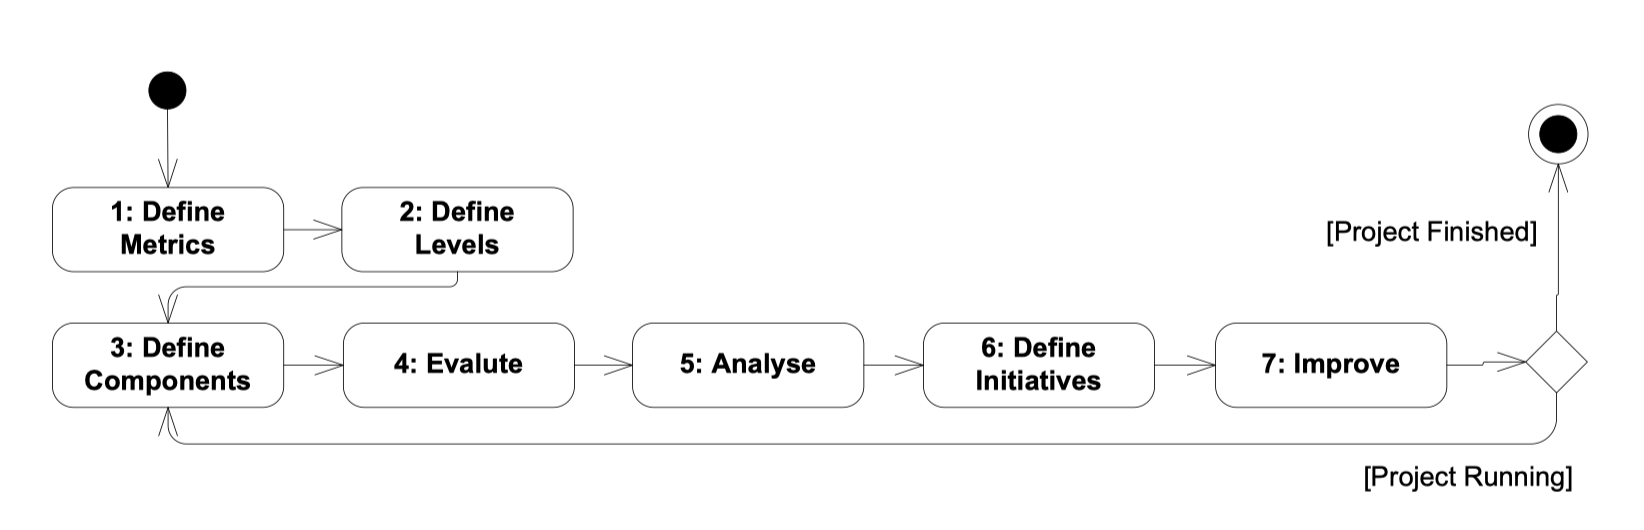
\includegraphics[width=0.7\textwidth]{thesis/latex/assets/asqa-process-steps.png}
    \caption{aSQA Process Steps from \cite{asqa-paper}}
    \label{fig:asqa-process-steps}
\end{figure}

\begin{enumerate}
    \item \textbf{Define Metrics} to the components of the system. This can be done with \glspl{qas}, which may define the desired quality.
    \item \textbf{Define Levels} to measure the state of the system
    \item \textbf{Define Components} to scope the parts of the system that will be evaluated
    \item \textbf{Evaluate} by taking the scenarios and looking at the architecture of the system. An evaluation matrix is used to define the following levels: (t)arget, (c)urrent, (health), (i)mportance, (f)ocus
    \item \textbf{Analysis} will look at the areas where the value of focus is high
\end{enumerate}

\vspace{0.5cm}
\paragraph{Metrics}\mbox{}\\

The defined \glspl{qa} are helpful to know but cannot be tested, or often qualities of a system are hard to categorize with an adequate \gls{qa}. A solution to the problem of untestability and overlapping concerns is \glspl{qas}. \glspl{qas} can be used to characterize \glspl{qa} \cite{BassSoftwareArchitecture2003}. Based on the scenarios, the evaluation will be carried out. The scenarios will always have the \glspl{qa} in mind and are defined with the focus on those. The different scenarios are predicted to be the most common actions on the system and will stress the design and its architecture the most based on the \glspl{qa}.

The previously picked \glspl{qa} are as follows:

\begin{enumerate}
    \item Security
    \item Performance
    \item Usability
\end{enumerate}

Possible scenarios are centered around data not being available or altered or scenarios of malicious behavior from an adversary by injecting code to misuse the system in unintended ways:

\begin{enumerate}
    \item As a user, I expect after commenting to see my comment in Indico, but also in my data pod
    \item As a user, I expect after deleting my comment in my data pod that the comment is not shown in Indico
    \item As a user, I expect after I edit my comment in my data pod that the comment will be updated in Indico
    \item As a user, I expect to be able to revoke access to my data pod for the application
    \item As a user, I expect to see others' comments
    \item As a user, I expect only to give access to the necessary data
\end{enumerate}

\paragraph{Levels}\label{poc1-levels}\mbox{}\\

The levels are used to measure the state of the architecture of the system. These can be freely chosen but follow an ordinal scale ranging from 1 to 5 in the original paper and adapted \cite{asqa-paper}. The levels will help rate the quality of the system's architecture, where one is the lowest quality and five the highest rating.
\vspace{0.5cm}
\paragraph{Components}\mbox{}\\

To evaluate the security of the system's chosen architecture, it makes sense to look at specific components of the system. It would be sensible to analyze the \texttt{auth} package and the modules that interface the user input and the design for this commenting system. The user input modules can be found in the \texttt{component} package.

\begin{figure}[!ht]
    \centering
    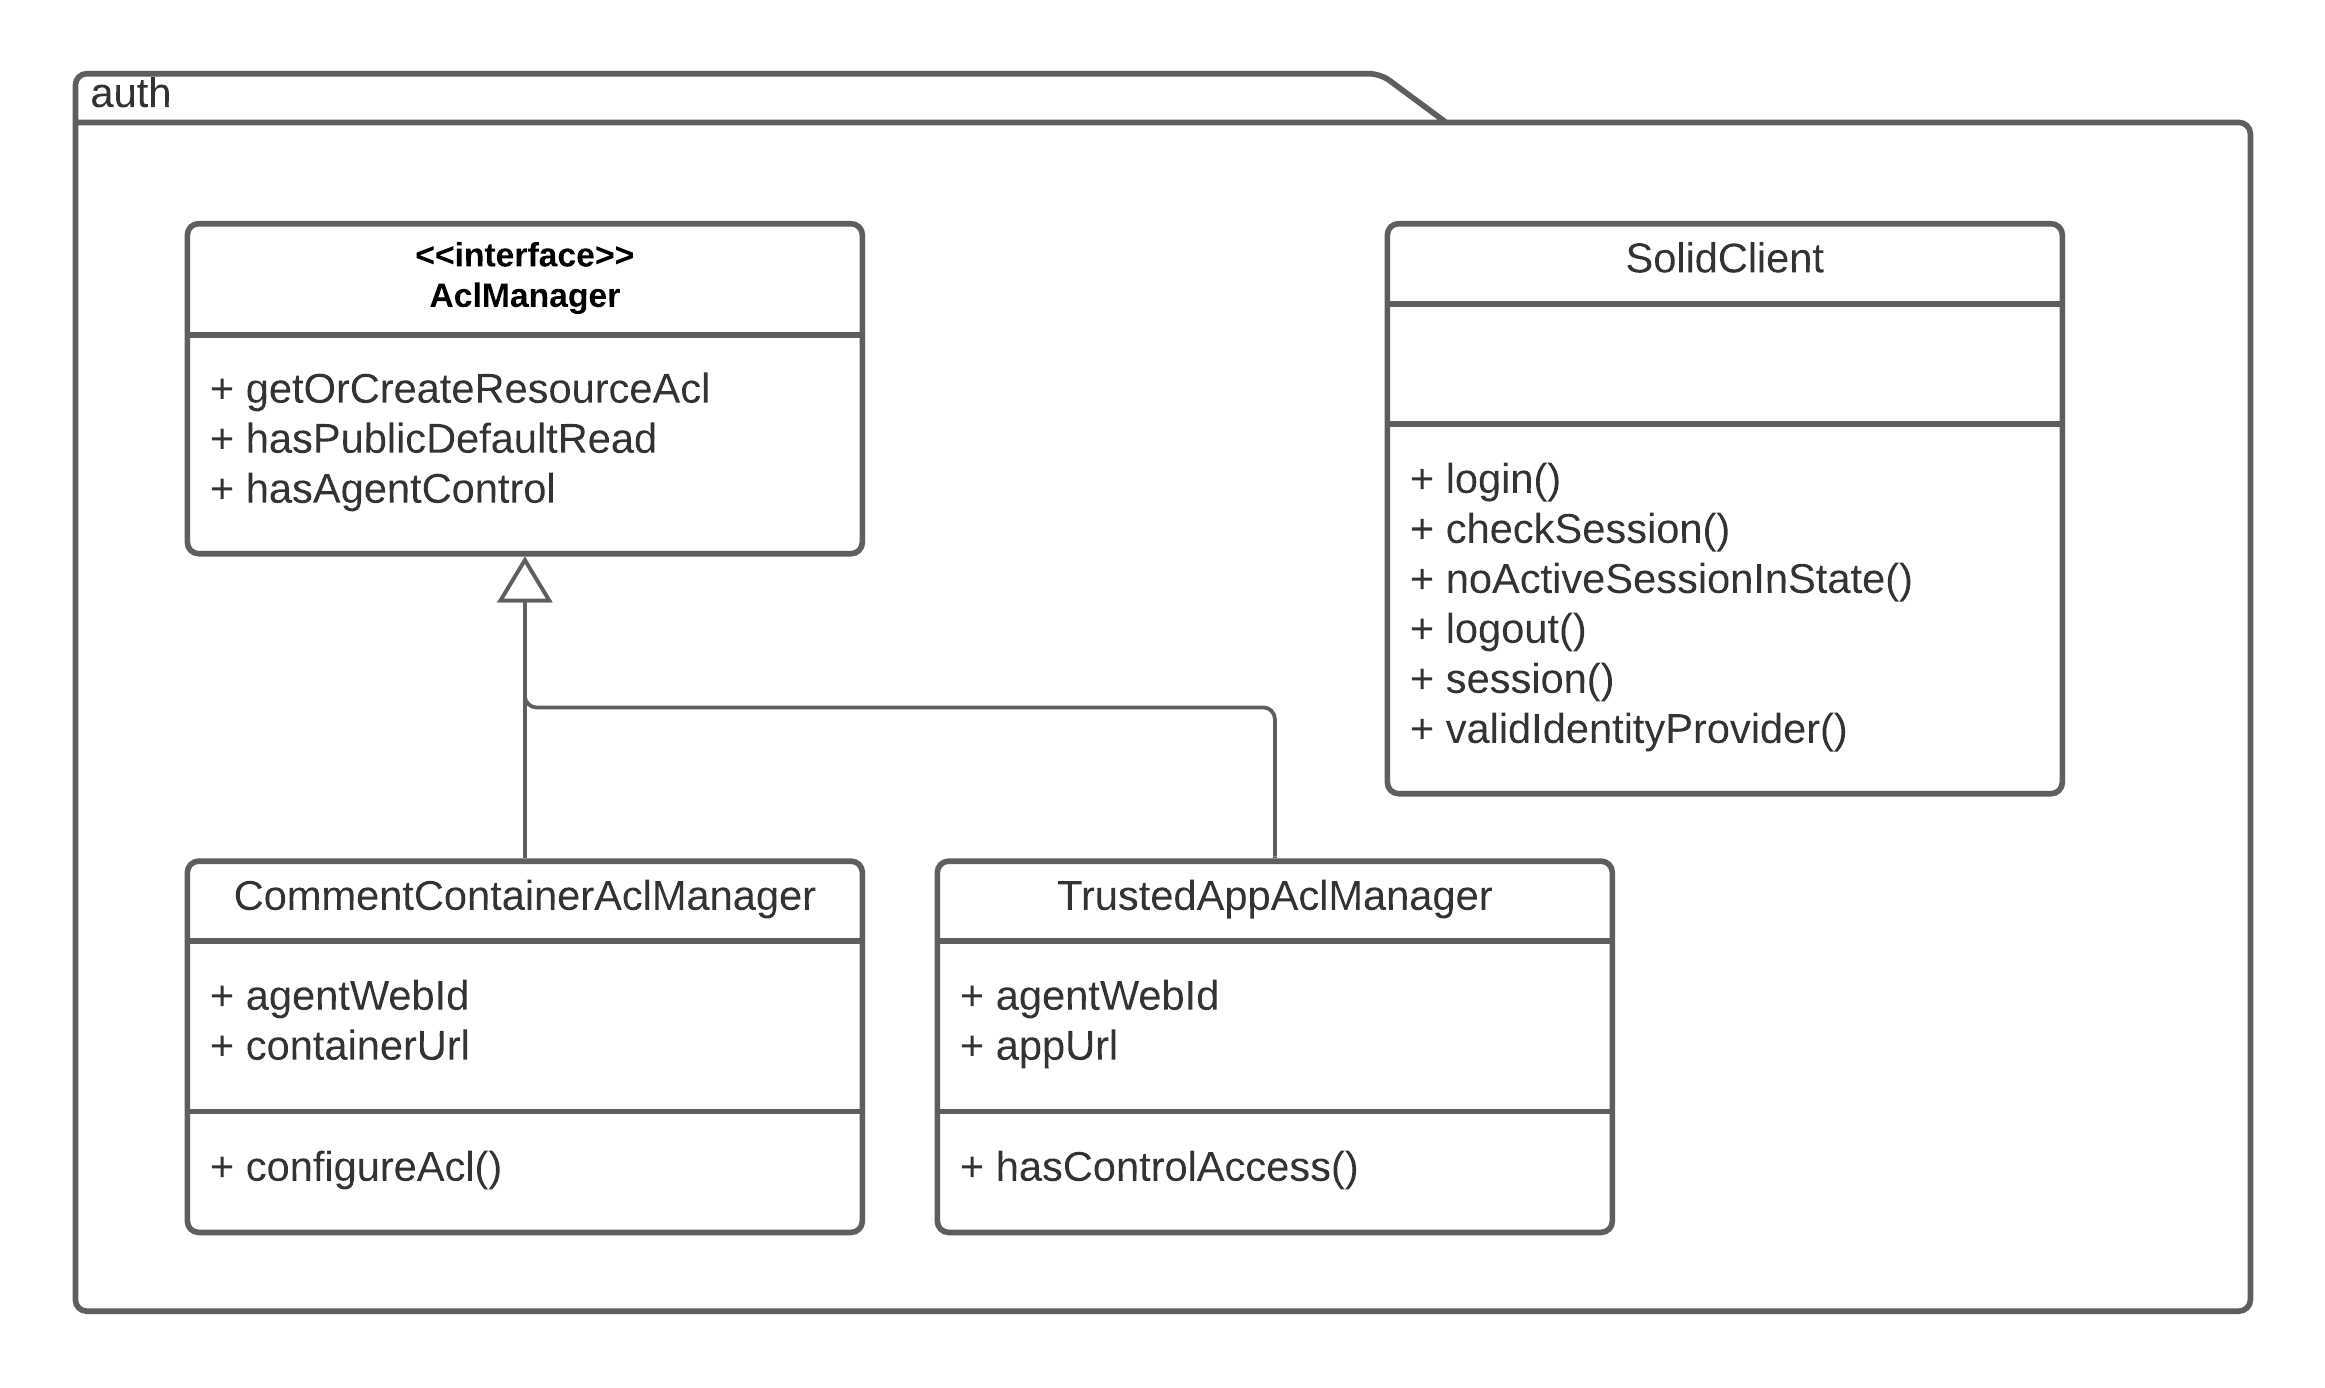
\includegraphics[width=0.7\textwidth]{prototype/graphs/poc-comment-package-auth.png}
    \caption{The \texttt{auth} package with its classes.}
    \label{fig:poc-comment-package-auth}
\end{figure}

The \texttt{auth} package holds classes handling the \gls{acl} logic necessary. The logic ranges from checking for existing specific authorization modes or creating new \gls{acl} files for resources and updating existing resources. A careless architecture could either give too much access control or allow privilege escalation, where a flaw in the software can be used to elevate the access modes for an adversary.

The \texttt{auth} package further holds the \texttt{SolidClient} class. The \texttt{SolidClass} is a wrapper class for the external authentication functions, which bring the authentication and session management for the Solid ecosystem. Naturally, all authentication modules need to be inspected and made sure no vulnerabilities are let in.

\begin{figure}[H]
    \centering
    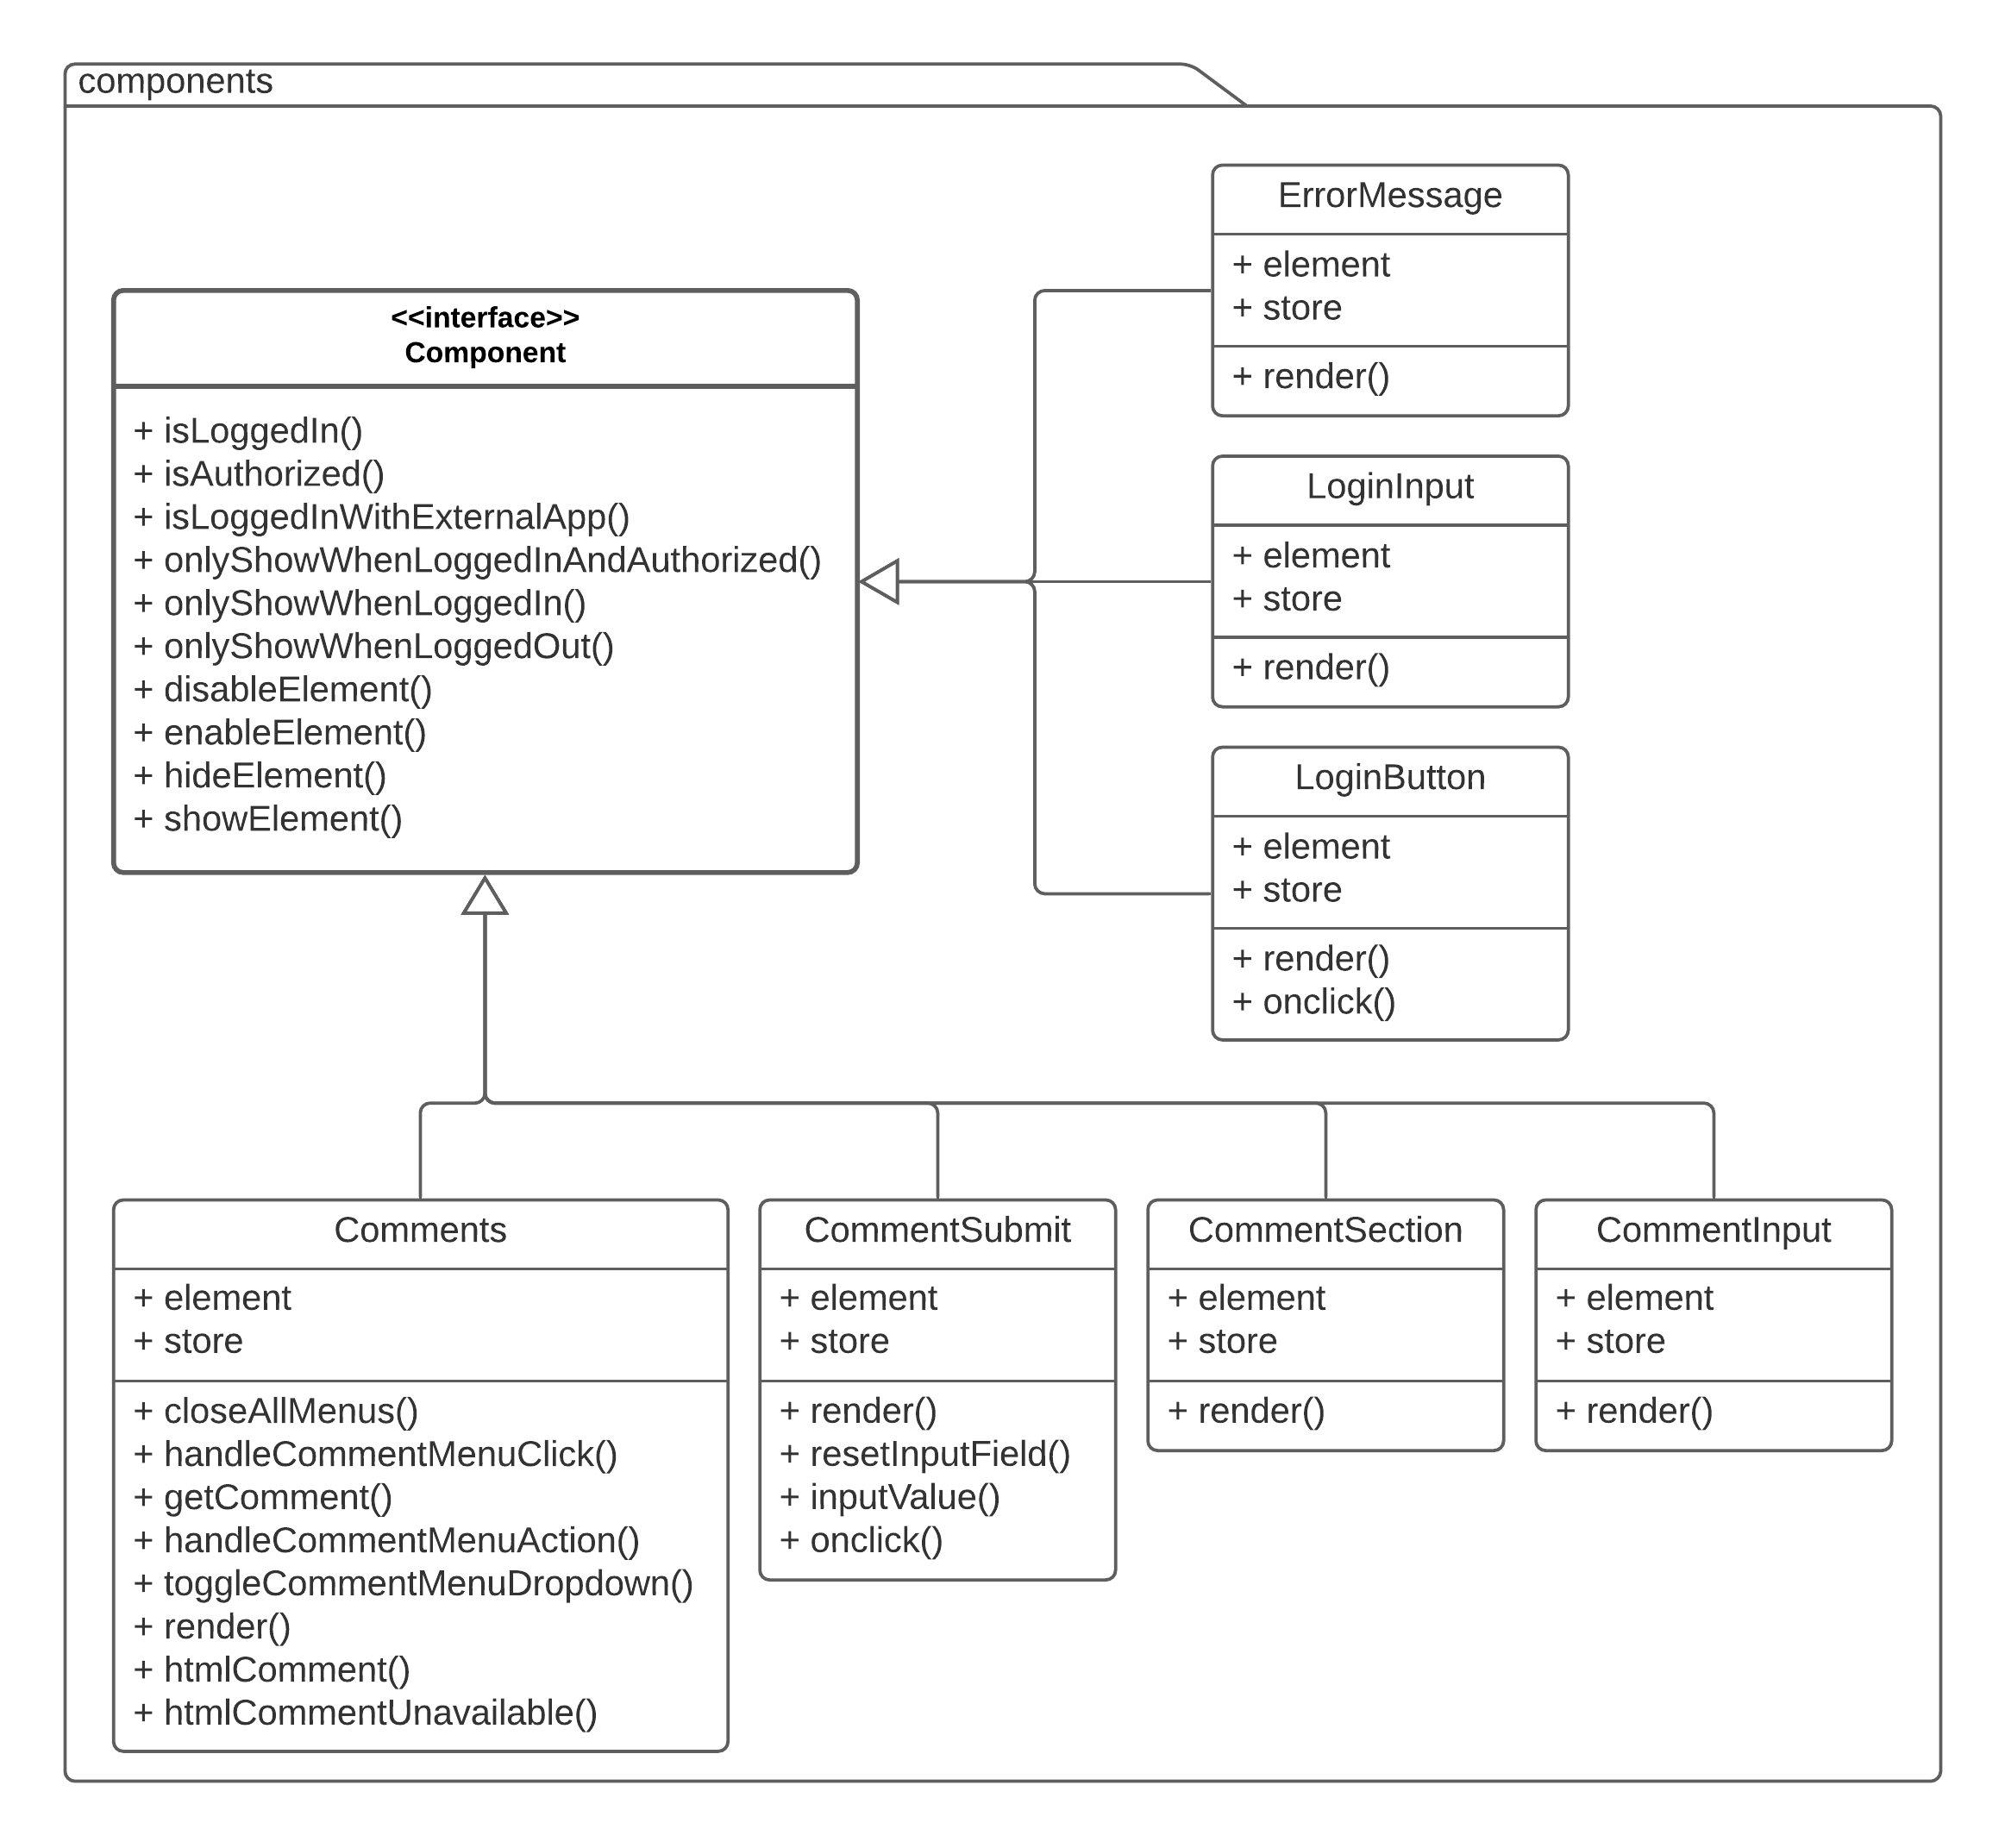
\includegraphics[width=0.7\textwidth]{prototype/graphs/poc-comment-package-components.png}
    \caption{The \texttt{components} package with its classes.}
    \label{fig:poc-comment-package-components}
\end{figure}

The second package, \texttt{components}, holds all elements in the \gls{ui} that have to interact with the state management module. These classes range from the input field for the WebID \gls{uri} to retrieve the address of the user's \gls{idp} to the rendered comments.
% During a first iteration through the evaluation of the architecture it was established that splitting up and looking at the modules separately does not make sense in this case. Most of the time -- no matter -- which scenario is looked at all modules are being stressed. Often, the values would be the same even though another component was tried to be analyzed. Therefore, for the sake of simplicity and  
\vspace{0.5cm}
\paragraph{Evaluate}\mbox{}\\

\begin{itemize}
    \item \textbf{Target}: What is the desired quality level?
    \item \textbf{Current}: What is the current level?
    \item \textbf{Health}: Where are the most considerable quality problems?
    \item \textbf{Importance}: How important is it to move from current to target level?
    \item \textbf{Focus}: What are the most significant and most essential quality problems?
    \item \textbf{Valid level values}: 1, 2, 3, 4, 5 (higher equals better)
\end{itemize}

\textbf{Health} and \textbf{focus} are not set by the evaluator but instead calculated from other levels.

\begin{align*}
    \text{\textit{health}}&=5 - \text{\textit{max}}(0, (\text{\textit{target}} - \text{\textit{current}}))
\end{align*}
\vspace{-5mm}
\begin{align*}
    \text{\textit{focus}}&= \text{\textit{ceil}}((6 - \text{\textit{health}}) * \text{\textit{importance}}/5)
\end{align*}

\begin{enumerate}
    \item A user logs in with their WebID and posts a comment
    \item An adversary posts a comment with a string containing a \gls{xss} attack
    \item High load of traffic is occurring with comments being posted within seconds
    \item An adversary deploys software on their pod to serve varying resources based on the geolocation of the connecting \gls{ip} address
\end{enumerate}

\begin{table}[h!]
    \centering
    \begin{tabular}{| l | c | c | c | c | c |} 
     \hline
     \texttt{auth} & T & C & H & I & F \\
     \hline
     Security & 5 & 2 & 2 & 5 & \cellcolor{red!25}4\\
     \hline
     Performance & 5 & 1 & 1 & 5 & \cellcolor{red!50}5\\
     \hline
     Availability & 4 & 3 & 4 & 2 & \cellcolor{green!25}1\\
     \hline
     Usability & 5 & 2 & 2 & 4 & \cellcolor{red!25}4\\
     \hline
    \end{tabular}
    \quad
    \begin{tabular}{| l | c | c | c | c | c |} 
     \hline
     \texttt{components} & T & C & H & I & F \\
     \hline
     Security & 5 & 3 & 3 & 5 & \cellcolor{orange!50}3\\
     \hline
     Performance & 5 & 1 & 1 & 5 & \cellcolor{red!50}5\\
     \hline
     Availability & 4 & 3 & 4 & 2 & \cellcolor{green!25}1\\
     \hline
     Usability & 5 & 3 & 3 & 3 & \cellcolor{green!25}2\\
     \hline
    \end{tabular}
    \vspace{0.75cm}
    \caption{Evaluation of the two packages based on the \glspl{qas}}
    \label{table:poc1-evaluation}
\end{table}

\subsubsection{Analysis}\mbox{}\\

The following analysis section will explain how the values of the two tables from \ref{table:poc1-evaluation} came together and will give some more insights into how the modules are working and behaving in certain situations. After the explanation and analysis of this particular evaluation a broader analysis of the \gls{poc} will be given, where critical areas in the architecture will be highlighted and some possibilities for future iterations of it.
\vspace{0.5cm}
\paragraph{\texttt{auth} and \texttt{components} packages}\mbox{}\\

The \texttt{SolidClient} class is part of the \texttt{auth} component package, which handles the session management. When the comment module is loaded upon page load it is \textit{booted} with the flow shown in \ref{fig:poc-comment-flow-app_boot}. It can be observed that every time the module is loaded it has to do four round trips to the \gls{idp} and data pod. Once the application is booted, the list of comment \glspl{uri} are passed to the application and it fetches all comments from their remote data pods. This behavior is linked to the \texttt{components} module, as it is responsible for rendering all these comments in the \gls{dom}. Further performance analyses in regards to the fetching of the comments is being done below in the paragraph \ref{paragraph:evaluation-performance}. But when the comments are being fetched a second request happens that loads the WebID profile of the author of the comment. Resulting in $n*2$ requests, where $n$ is the number of comments. The exact flow of getting the comments is shown in figure \ref{fig:poc-comment-flow-set_comments}.

\begin{figure}[H]
    \centering
    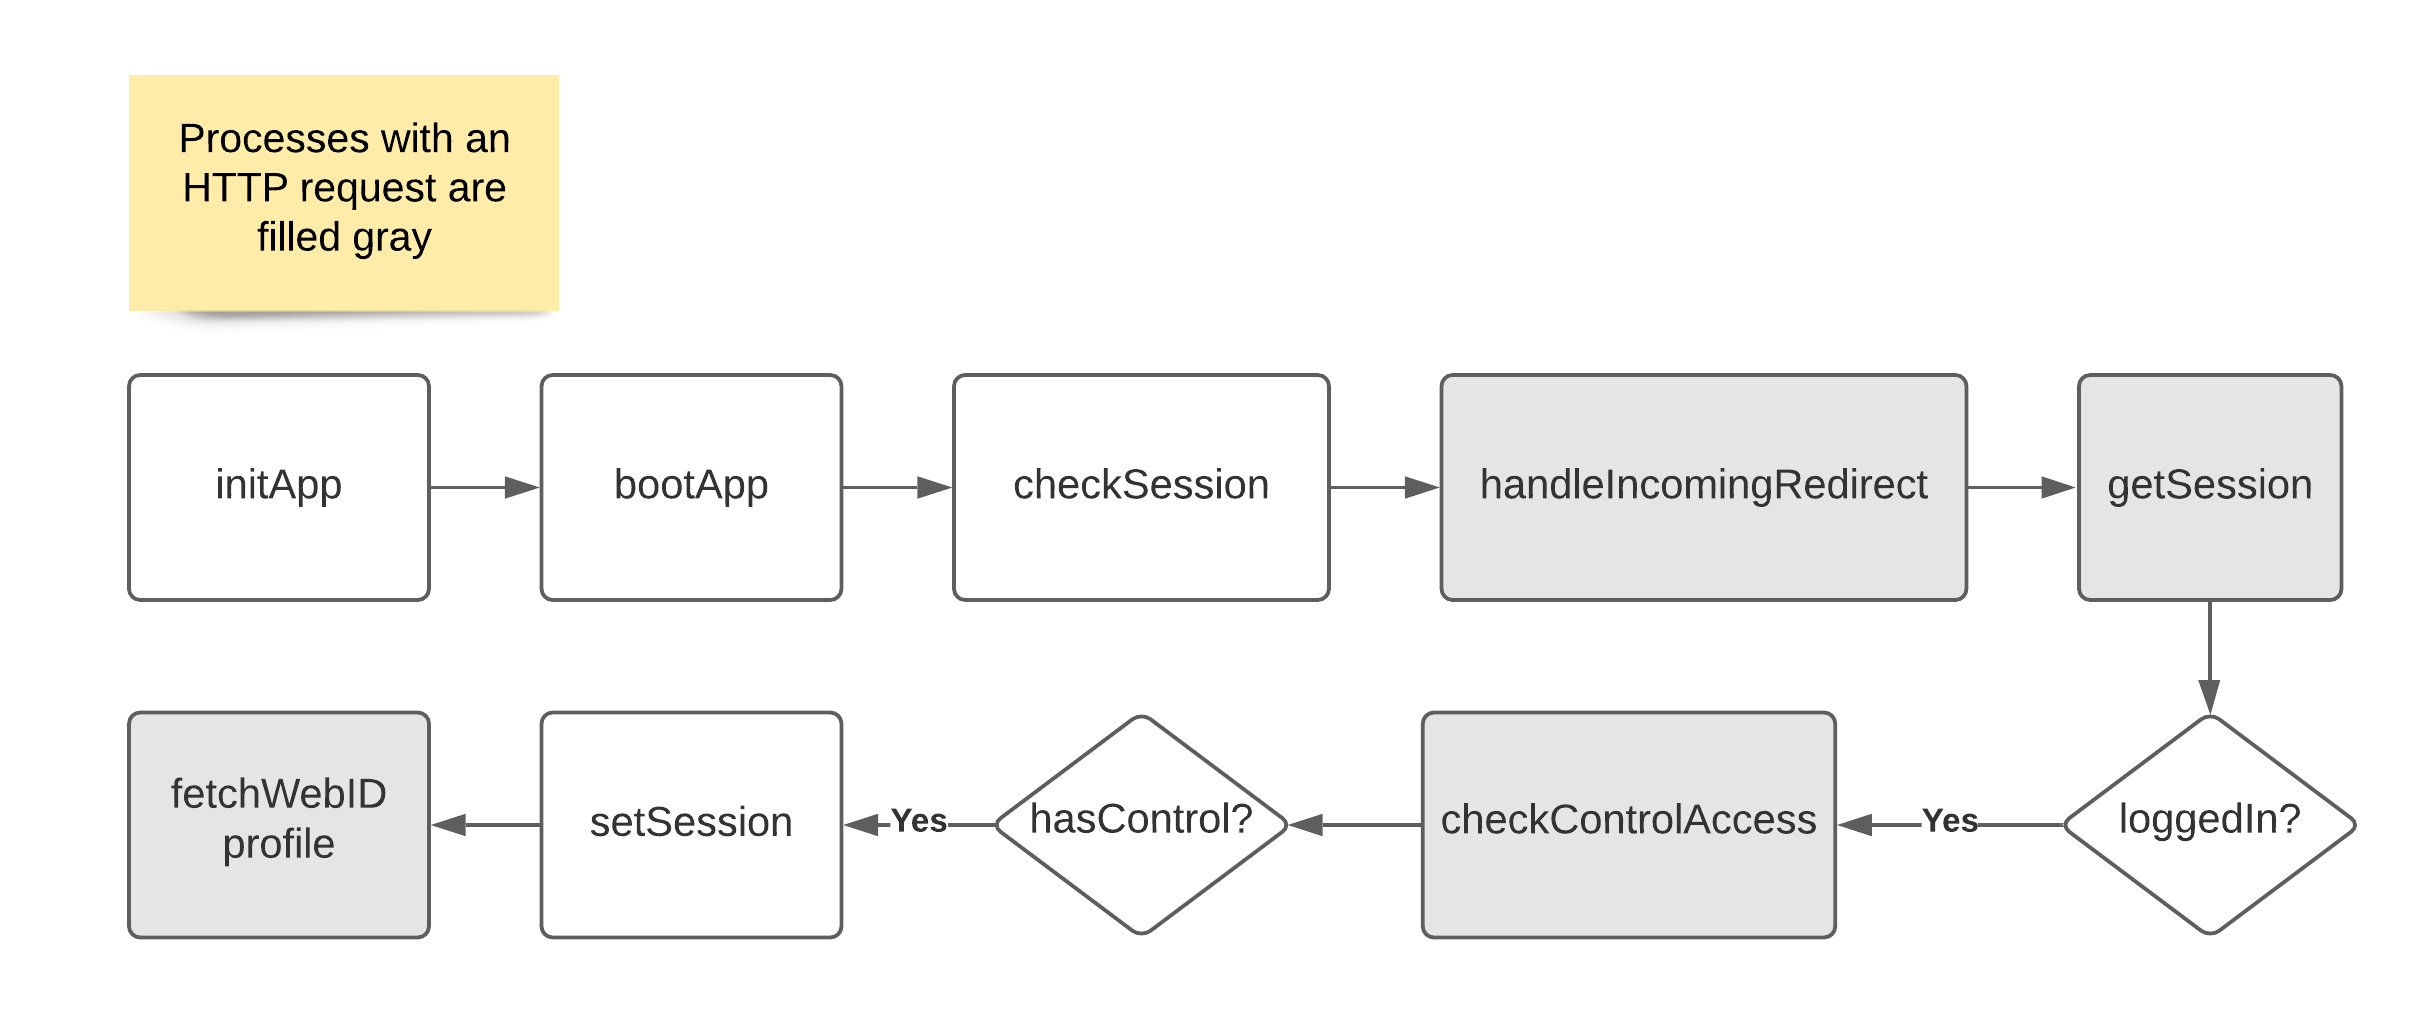
\includegraphics[width=0.7\textwidth]{prototype/graphs/poc-comment-flow-app_boot.png}
    \caption{Application boot flow. External \gls{http} requests are indicated by a filled grey box.}
    \label{fig:poc-comment-flow-app_boot}
\end{figure}

\begin{figure}[H]
    \centering
    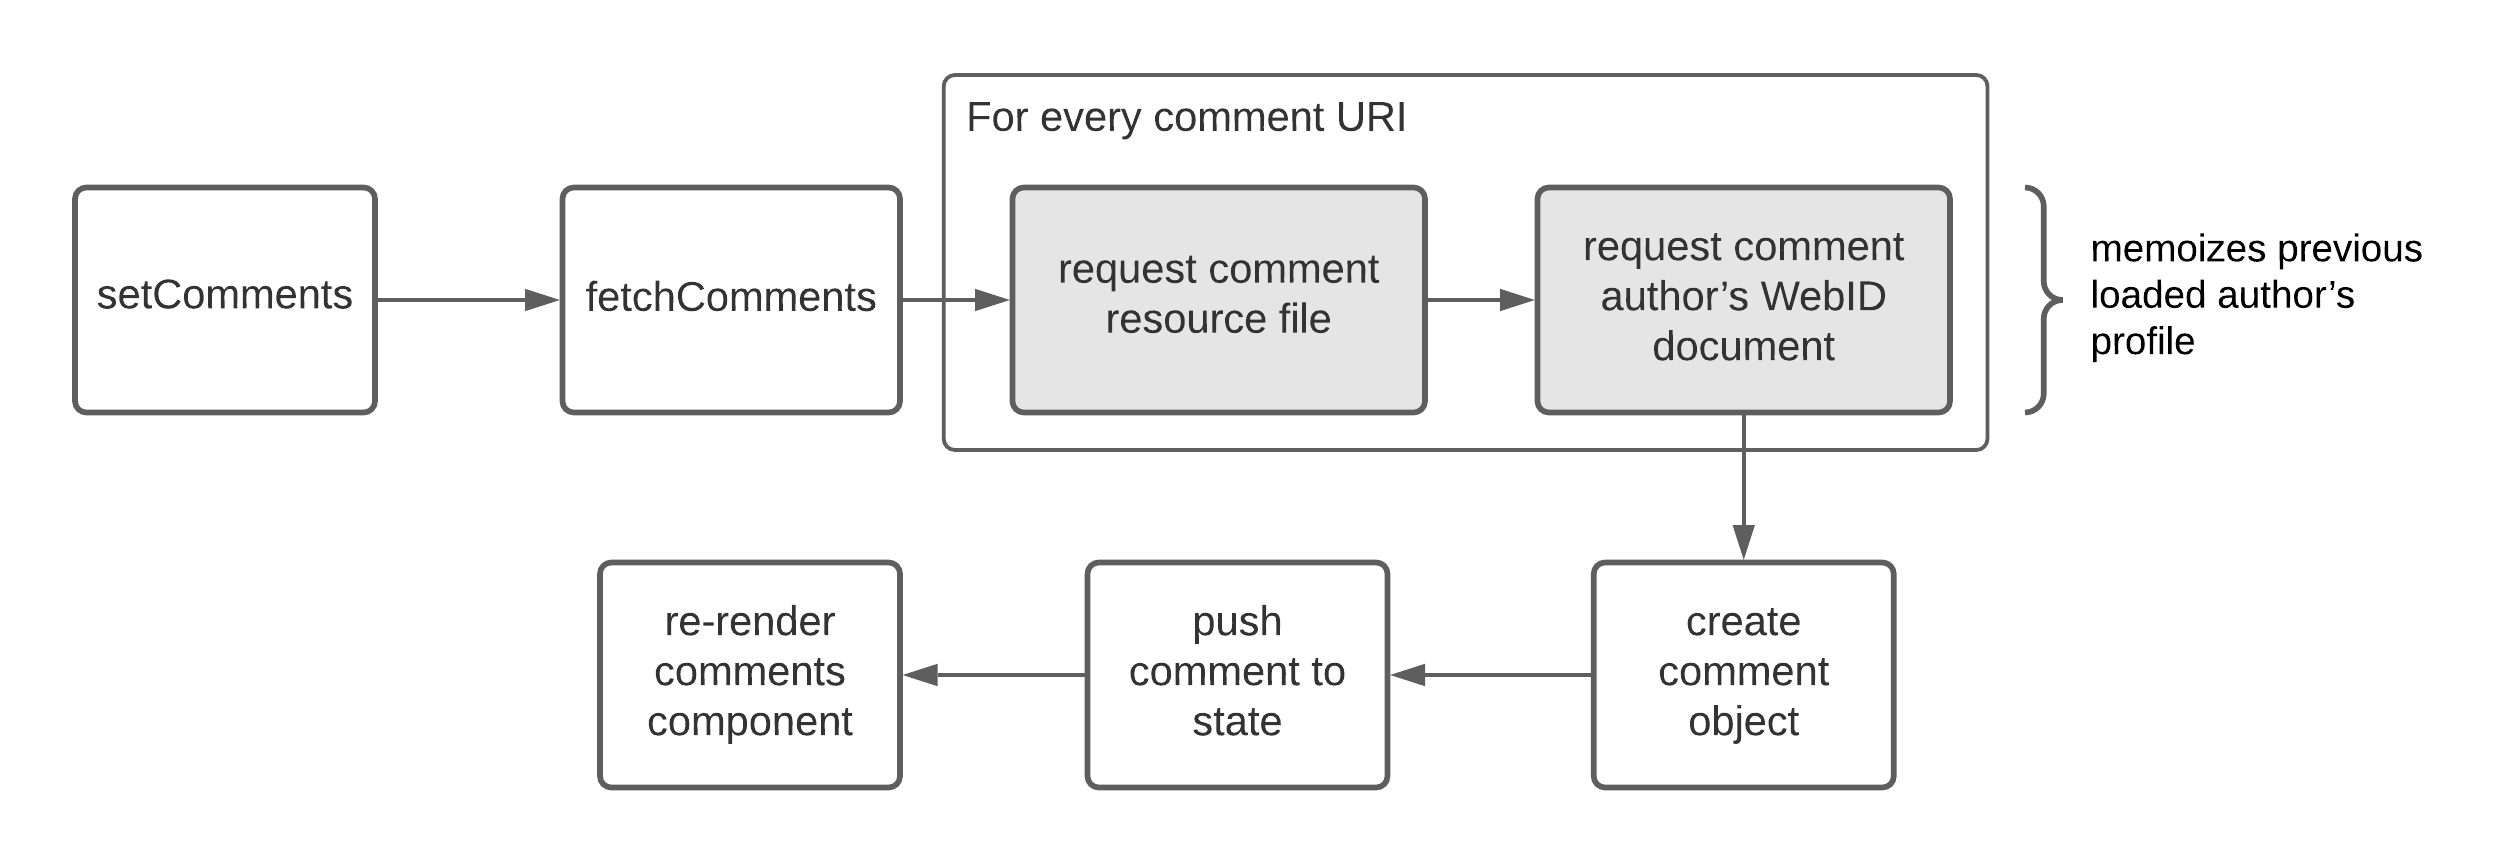
\includegraphics[width=0.7\textwidth]{prototype/graphs/poc-comment-flow-set_comments.png}
    \caption{Requesting comments from data pod. External \gls{http} requests are indicated by a filled grey box.}
    \label{fig:poc-comment-flow-set_comments}
\end{figure}

The application boot with successive comment fetching happens every time the system is loaded, which is in minimum four requests, when no comments are loaded and $n*2+4$ requests with $n$ comments.

In regards to \textit{availability} for both looked at modules if a data pod is unavailable the \texttt{auth} module will simply not be able to do its checks on whether a session is present. The \gls{http} requests checking the session will respond with $40x$ \gls{http} status codes and simply disallow any comment posting. For the \texttt{components} module a dedicated message has been implemented which will render a hint on why a comment may not have loaded when a data pod is unreachable. The hint renders one long message guessing what has happened, but is not clever about inferring the reason.

\begin{figure}[H]
    \centering
    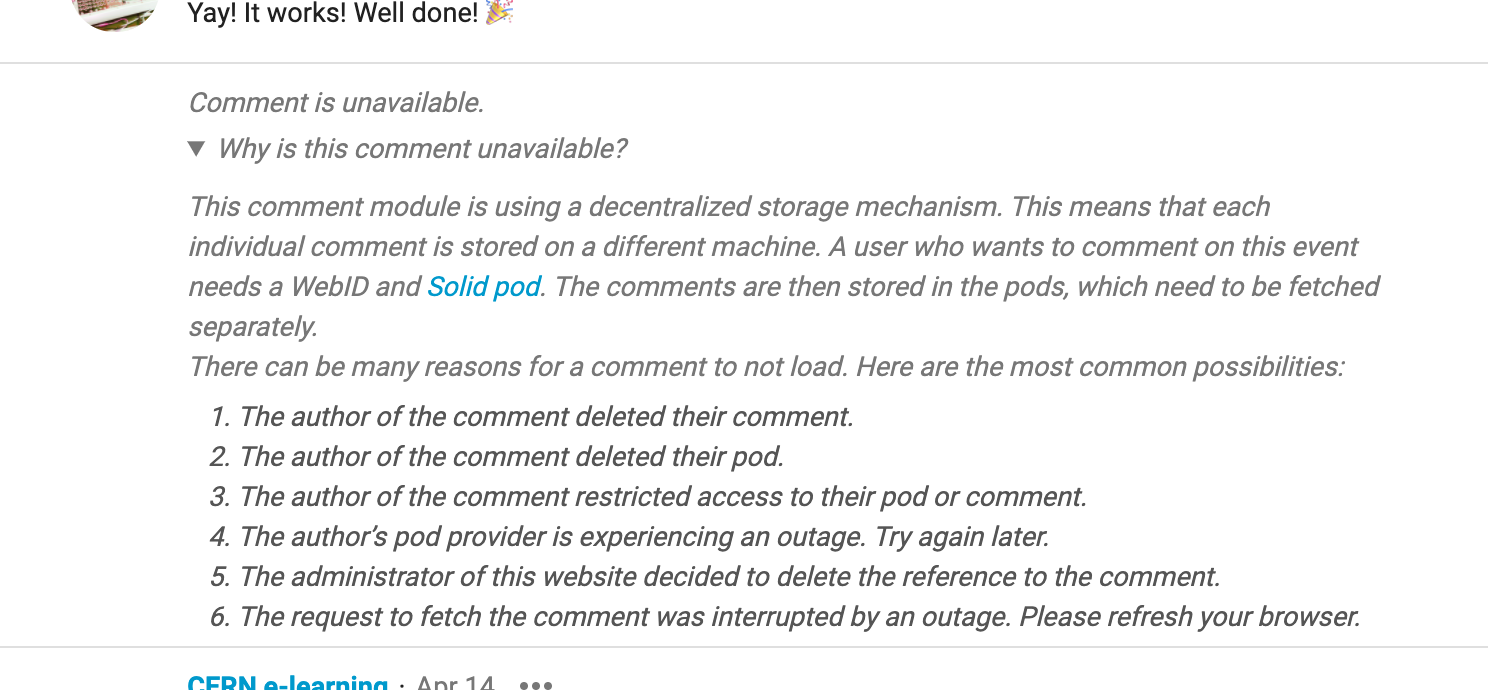
\includegraphics[width=0.7\textwidth]{prototype/poc-comment-unavailable_comment.png}
    \caption{Hint when a comment could not be loaded}
    \label{fig:poc-comment-unavailable_comment}
\end{figure}

Another striking value is the high focus for the usability in the \texttt{auth} component. This can be explained with the fact that it is not made clear to the user that \textit{control} access to the root container of the data pod is needed in order for the application to function properly. Only when an authenticated session from the Solid \gls{idp} is present and the \textit{control} access is lacking it will show in the interface. Firstly, this results in a bad user experience, but more over the fact that the user needs to gives full control over the data pod to the application is unfortunate. The end-user who is not a Solid professional will have a hard time understanding the reason and may step back from application that need this much control. The evaluation for the \textit{security} resulted therefore also with a worse level than it could have scored. The security within the module is relatively stable with sanitization of inputs not allowing any malicious code to be executed when fetching resource from data pods.

\vspace{0.5cm}
\paragraph{Performance}\label{paragraph:evaluation-performance}\mbox{}\\

The chosen technique of storing the comments is not as efficient as it could be. Every comment is stored as a self-contained Turtle file on the author's comment with Indico holding the \gls{uri} to be able to fetch it on demand. As soon as the client is loading the module with the comments the client will have to make $n$ requests, $n$ being the number of comments.

The first improvement to this approach could be pagination. Pagination limits the number of initially loaded comments to a defined amount. This can be achieved by utilizing the date and time from the file name of the comment. Only the most recent $n$ comments by time will have to be fetched. When the user clicks on a load more comments button, $n$ more comments will be loaded.
In the same area of improvement, the ways the comments are rendered can also be improved. The comments as of now will all be fetched and only when all requests are done it will be rendered in the \gls{dom}. If the comments are \textit{separated} from each other and a comment is rendered as soon as it successfully fetched, it would speed up the time until a user could start seeing comments.

The second improvement could be a grouping of comments by the author. This way the number of requests would now be bound to the number of authors. In the worst case, where all comments are from different authors, it would not bring any improvement over the initial architecture. The design for this would be to change the storage from the multi-file approach to a single-file approach. On the data pod, one file would exist holding all comments from one author for one event. This file can be fetched with one request containing multiple comments.
% Another way of achieving this is to use a more efficient asset providing web protocol, such as \gls{http}/2. \gls{http}/2 uses a clever technique to 

Another enhancement can be attained by caching. In its current design, the comments are freshly fetched on each page load. Server-side \gls{http} caching is out of control for the clients, and completely relies on the Server implementations to do so. By Solid specification, \gls{http} caching is prescribed, but not vital \cite{solid-protocol}, which means it \textit{should} implement it, but does not have to. Regardless, the improvement would not be in the number of round trips the client has to complete, but rather in the time for the server to calculate the response it sends out \cite{http-caching}. A real improvement on consecutive page visits are won by client-side \gls{http} caching. Upon successive visits to a cached website, a previously fetched and in the browser's local storage stored copy of the response would be served \cite{http-caching}. The result would be immediately loaded, but might not serve the latest and up-to-date asset from the server. The \textit{freshness} of the response is controlled using the \texttt{Cache-Control} header in either the request or response of the \gls{http} exchange between client and server \cite{http-caching}. 

More performance solutions shall be looked at with the other upcoming areas in this analysis section.
\vspace{0.5cm}
\paragraph{Security: Modification of Resources}\mbox{}\\

In the case of comments being the resources that are being shared between data pod and application, it has been established a modification from outside the application is acceptable behavior. For a resource where a modification should be monitored or even forbidden. A few paths are conceivable.

Storing the comments on the author's data pod could be given up and instead be done by a trusted entity, e.g. the application embedding the comment module. It would result in \gls{cern} hosting one data pod for their Indico instance. Each event would create a container in this data pod with \textit{append} access mode for the public. \textit{append} allows an agent to add new resources to a container, but not modify or delete any \cite{solid-protocol}. Through this access mode a user can post comments freely, but cannot modify them at a later stage, as the data is now in Indico's data pod and the user is lacking the access control to edit existing resources. Having one data pod responsible for all comments also improves the performance by reducing the number of \gls{http} requests needed. Whereas before the requests were either bound to the number of authors or even by the number of comments, it is now only a single request to the event's container on the Indico data pod, to fetch a single file with all comments written in. A drawback to this approach is the comments are again stored centralized in one storage, though because it is using a Solid server instead of a web server with unstructured data storage, the data is now structured and thus interoperable through \textit{Linked Data}. Besides storing it in Indico's data pod, a copy of the comment could be stored in the author's data pod. The author acquires a version of the comment and Indico holds the \gls{ssot}.

One more option to control the modification on resources while not giving up on decentralized storage in the author's pods is to use versioning on the comments. Indico would when a user creates and submits a comment store a hashed value of the comment's content. When then serving the comments from the external data pods to visiting clients the received comments would be hashed and compared to the Indico stored hash value. It is important to associate the comment's \gls{url} with the hash to be able to make a proper comparison on the correct resources.

An important aspect of allowing the update of existing resources is to have an indication in the \gls{ui} notifying readers about a changed text. A simple \textit{edited}-hint would suffice. When a user is browsing the comments and follows a conversation, which is met with an abrupt disruption of flow in the conversation, an updated comment could be the result and an indication would help to identify such a situation.  To detect a change in the comment's content the same hashing function can be used as described before.
\vspace{0.5cm}
\paragraph{EventSettingsProxy Scalability Issues}\mbox{}\\

The implementation with EventSettingsProxy is not scalable and a production-ready technique. Even though transactions are being used in the database and a dedicated table is being used to persist all related settings for the events, it can still happen that race conditions occur. As for example two requests read the event settings table and retrieve an entry with $[1,2]$ for the column holding the list of comment \glspl{url}. When request A now writes $3$ and request B write $4$ it generate two \gls{sql} \texttt{UPDATE} statements, one with $[1,2,3]$ and one with $[1,2,4]$ where the second overwrites the first and only $[1,2,4]$ is persisted.

Justification for implementing it in this way is a faster \textit{time-to-market} allowing a quicker development and thus testing of the prototype. It was never expected to test the prototype where these race conditions would occur. If a production-ready module should be developed, a separated database table would need to be created and every new comment \gls{uri} would be added to the database by using \gls{sql} \texttt{INSERT} statement, which are safe against race conditions. A further benefit would be the ability to store more comment specific meta information such as signatures or hash values to be able to detect changes in pulled in comments.
\vspace{0.5cm}
\paragraph{Indico Solid Proxying}\mbox{}\\

Indico could develop an \gls{api} which sits between Indico and the Solid data pods to then for example make all the requests on behalf of the clients. A proxy as such would hide all the clients' \gls{ip} addresses and would therefore disallow the logging of client \gls{ip} addresses by a malicious data pod. A performance improvement is also foreseeable as the Indico proxy could make the requests to the different data pods and put them into cache where they would then be served from. By caching the request in this layer, the request do not have to be made by every client every time on page load. Loading resources before they are requested by clients and then serving clients from a cache is called cache warming \cite{cache-warming}. Another benefit of doing the requests using an Indico proxy is also that a malicious data pod or just one that wants to do some kind of targeted advertisement, cannot identify the clients by their \gls{ip} addresses and therefore not send different responses upon requests from different \gls{ip} addresses based on geolocation.
